
\documentclass[a4paper,12pt]{article}
\usepackage[toc,page]{appendix}
\usepackage{amsmath}
\usepackage{geometry}
\usepackage{graphicx}
\usepackage{subcaption}
\usepackage{multirow}
\geometry{margin=1in}
\graphicspath{ {Images/} }
\begin{document}


%%%%%%%%%%%%%%%%%%%%%%%%%%%%%%%%%%%%%%%%%%%%%%%%%%%%%%%%%%%%%%%%%%%%%%%%%%%%%%% TITLEPAGE
\pagenumbering{gobble}
\centering
\vspace*{5cm}
{\huge Developing AntBot: \par Visual Navigation based on the insect brain \par}
\vspace{1cm}
{\itshape Robert Mitchell}

\vspace{2cm}

{\large Master of Informatics \par}
{\large Informatics \par}
{\large School of Informatics \par}
{\large The University of Edinburgh \par}
\large \today \par

\vfill
Supervised by\par
Dr. Barbara Webb

\newpage

%%%%%%%%%%%%%%%%%%%%%%%%%%%%%%%%%%%%%%%%%%%%%%%%%%%%%%%%%%%%%%%%%%%%%%%%%%%%%%% ACKNOWLEDGEMENTS
\pagenumbering{roman}
\centering
{\LARGE \textbf{Acknowledgements}}
\begin{flushleft}
 {\small
  I would like to take the opportunity to thank my supervisor, Dr. Barbara Webb, for her
  guidance, and invaluable insight on the subject matter. My gratitude also extends to
  Zhaoyu Zhang and Leonard Eberding, two of my predecessors on this project; both have been
  extremely useful in explaining the existing codebase and operations of the robot where they
  were not always clear. Finally I should like to thank my parents, for their unwavering support
  throughout my education; I could not have made it here without them. }
\end{flushleft}  

\newpage
%%%%%%%%%%%%%%%%%%%%%%%%%%%%%%%%%%%%%%%%%%%%%%%%%%%%%%%%%%%%%%%%%%%%%%%%%%%%%%% ABSTRACT
\centering
{\LARGE\textbf{Abstract}}
\begin{flushleft}
  {\small \textit{The abstract will be written as one of the last parts of the report to allow
    an accurate summary of the project as a whole.}}
\end{flushleft}

\newpage

%%%%%%%%%%%%%%%%%%%%%%%%%%%%%%%%%%%%%%%%%%%%%%%%%%%%%%%%%%%%%%%%%%%%%%%%%%%%%%% DECLARATION
\centering
{\LARGE\textbf{Declaration}}
\begin{flushleft}
  {\small
    I declare that this disseration was composed by myself, the work
    contained herein is my own except where explicitly stated otherwise
    in the text, and that this work has not been submitted for any other
    degree or professional qualification except as specified.
    \par 

    \textit{Robert Mitchell}}

\end{flushleft}

\newpage
%%%%%%%%%%%%%%%%%%%%%%%%%%%%%%%%%%%%%%%%%%%%%%%%%%%%%%%%%%%%%%%%%%%%%%%%%%%%%%% CONTENTS


\tableofcontents

\newpage

%%%%%%%%%%%%%%%%%%%%%%%%%%%%%%%%%%%%%%%%%%%%%%%%%%%%%%%%%%%%%%%%%%%%%%%%%%%%%%% FIGURES
\listoffigures
\newpage

%%%%%%%%%%%%%%%%%%%%%%%%%%%%%%%%%%%%%%%%%%%%%%%%%%%%%%%%%%%%%%%%%%%%%%%%%%%%%%% TABLES
\listoftables
\newpage
%%%%%%%%%%%%%%%%%%%%%%%%%%%%%%%%%%%%%%%%%%%%%%%%%%%%%%%%%%%%%%%%%%%%%%%%%%%%%%% BODY
%%%%%%%%%%%%%%%%%%%%%%%%%%%%%%%%%%%%%%%%%%%%%%%%%%%%%%%%%%%%%%%%%%%%%%%%%%%%%%% INTRODUCTION
\pagenumbering{arabic}

\raggedright
\section{ Introduction }
Desert ants (\textit{Cataglyphis velox}) have the
remarkable ability to navigate through complex natural environments, using only low-resolution
visual information and limited computational power. It is well documented that many species of
ant, and other hymenoptra are capable of very robust visual navigation; however, it is as yet
unclear how the insects perform this seemingly complex task with such little brainpower. In this
paper, we will focus on using and extending an existing model for visual navigation in ants using
the Mushroom Body circuit, an artificial neural network which emulates the Mushroom Body neuropils
in the ant brain. We will also discuss biologically plausible methods of visual Collision Avoidance
using Optical Flow. A robot (AntBot) has been constructed \cite{Eberding2016} to allow us a testing
platform on which to implement, and experiment with, the algorithms in the
\textit{Ant Navigational Toolkit} \cite{Wehner2009}.

\subsection{ Motivation }
Though we are able to observe and mimic algorithmically the visual navigational capabilities
of insects, we still do not understand the precise methods by which this process takes place. The
model we will look at was propsed by \textit{Ardin et al.} \cite{Ardin2016}, which takes
the Mushroom Body (whose function was thought to be primarily for olfactory learning), and shows
that this provides a plausible neural model for encoding visual memories.
\newline

The MB circuit has been implemented and tested on AntBot by Eberding and Zhang respectively, however
the existing MB circuit is fairly simple. It uses binary weightings for the connections between
the visual projection neurons and the Kenyon Cells, and a single boolean Extrinsic Neuron denoting
image recognition. A modification was made by Zhang, whereby eight ENs were used, one for each of
the cardinal directions in the Central Complex model. This will be discussed further in
\ref{MBBackground}. The reader should note that the Central Complex (CX) model is primarily used
to model the task of Path Integration and will not be discussed further (see \cite{Scimeca2017}).
\newline

We would also like to look at methods for collision avoidance (CA) which do not involve specialised
sensors such as a LIDAR or SONAR, the luxury of which, ants do not have. Models have been proposed
which use Optical Flow (OF) properties to determine whether or not a collision is imminent. These
models have been propsed both in purely robotic contexts \cite{Souhila2007},
and biological ones \cite{Low2005}. 
  
\subsection { Goals }
% EDIT: The reverse route may not be worth talking about, or perhaps integrated path integration?
% I'm not sure there is enough time for this

The project aims for the following experimental scenario to be possible: We want to send the robot
on a run through an obstacle course, allowing it to navigate however it chooses through the
environment. From here, we want the robot to be able to replicate this route using only visual
memories, which it should store on that initial run. Finally, we would like the robot to be able to 
navigate home following the reverse of this route. It should be noted that this final step is not
strictly accurate to the behaviour of the desert ant. As noted by \cite{Baddeley2012} in their
familiarity-driven study of ant route navigation, \textit{Wehner et al.} \cite{Wehner2006}
demonstrated that the remembered routes have a distinct polarity, so knowledge of a route from
nest to food, does not imply that the ant has knowledge of a route from food to nest. In this case,
we make the outward and homeward route the same.
\newline

The first stage of the project will focus upon obtaining a working collision avoidance system as a
pre-requisite to gathering the route information. This CA system should be based on visual
information readily available to AntBot with no additional/specialist sensors. For this paper, we
assume that CA is a low-level reactionary behaviour, in that, we do not use any further processing
of the detected motion; we react based on the immediate stimulus of the flow
field. We will look at two different optical flow techniques used to build CA systems. We will also
discuss the effects of using different types of flow field, how the different flow
techniques behave in the same situation, and different methods of response.
\newline

We then move to the Mushroom Body circuit; this model for visual navigation was demonstrated by
\cite{Ardin2016} in simulation. Previous iterations of this project which focussed on the Mushroom
Body circuit have struggled to achieve similar performance on a robot using the methods originally
presented by \textit{Ardin et al.}; certainly, no previous iteration
has dealt with a non-deterministic route through a cluttered environment. We aim to get the original
\textit{basic} model from \cite{Ardin2016} working on the robot in a robust fashion and hope to
establish a baseline agains which future iterations can work while modifying the model. We will use
a modified scanning behaviour to establish this baseline; ants have demonstrated use of scanning in
visual navigation but it is generally accepted that this
is not the primary method they use to determine a direction after having recognised a scene, rather,
this scanning behaviour only occurs in certain scenarios (e.g. when the ant becomes lost)
\cite{Kodzhabashev2015}. This will require debugging of the existing model and any interacting
factors; for example, \textit{Zhang} managed to achieve good results with the MB model using
klinokinesis as the route following behaviour while a scanning struggled to produce robust routes.
It should also be noted that the scanning behaviour performed poorly using a Perfect Memory model
(the highest performing model used by \textit{Ardin et al.}) which may suggest that the model is
not all that contributes to the accuracy of recapitulated routes.
\newline

Finally, we will report the results of the experiments and testing performed at different stages during, and
post development; we will compare these to relevant results from previous iterations of
this project. We will end with a conclusion of our findings and contributions to the project,
as well as discussing technical limitations and potential for future developments.
\newpage

\subsection { Results }
This work is based on work done previously by Leonard Eberding, Luca Scimeca, and Zhaoyu Zhang
\cite{Eberding2016, Scimeca2017, Zhang2017}.
\newline

Significant contributions:
\begin{enumerate}
  \item{An optical flow based system for Collision Avoidance,}
  \item{Results indicating the impracticality of a time-to-contact based system for Collision Avoidance,}
  \item{Implemented hardware upgrades to AntBot to make the platform more robust,}
  \item{Implemented a new type of scanning behaviour for AntBot,}
  \item{Successful replication of a route through a cluttered environment using Visual Navigation,}
  \item{Implemented a basic but extensible statistical logging utility on AntBot with a complementary parsing and plotting utility written in Python.} %AntBotStats
\end{enumerate}
\newpage

%%%%%%%%%%%%%%%%%%%%%%%%%%%%%%%%%%%%%%%%%%%%%%%%%%%%%%%%%%%%%%%%%%%%%%%%%%%%%%% BACKGROUND
\section{ Background}
\subsection{ Optical Flow }
\textit{Image flow} is defined as being the 3D velocity vector of an object, projected onto a
2D image plane\cite{ODonovan2005}. Optical flow is an approximation of this, working from a series
of images to compute the projected velocity vector for a pixel. A single \textit{flow vector}
shows the displacement of a single pixel from one image to the next. A set of these flow vectors
creates a \textit{flow field}, a series of vectors which describe the motion in the complete image.
\newline

Broadly, there are two types of flow field: dense and sparse (also known as differential and
feature-based repectively\cite{Low2005}). A \textit{dense} flow field tracks
the motion of every pixel in the image. A \textit{sparse} flow field tracks the motion of a subset
of pixels in the image. The sparse field may track a uniform subset of pixels, such as a grid, or a
set of important points in the image, such as the prominent features in the image (object corners).
See \ref{sec:methods} for implementation.


\subsection{ Optical flow models for Collision Avoidance } \label{sec:ofca}
Collision avoidance is an important component in navigation. Ants
do not have dedicated sensory systems or the ability to create a visual 3D map of their environment
using stereoscopic vision or motion paralax. It has been demonstrated that optical flow is used by
honeybees in performing visual navigation \cite{Dittmar2010}, so it is not unreasonable to
think that bees and other hymenoptera may use this information for other purposes. Indeed, optical
flow has been shown to be a viable model for collision avoidance in \textit{Drosophila}
\cite{Stewart2010}. We visit two models in this paper which we will term the
\textit{time-to-collision} model and the \textit{filtering} model.

\subsubsection{ Time-to-Collision }
This model, proposed by \textit{Low and Wyeth}\cite{Low2005}, aims to replicate the CA capabilities
of larger animals such as birds and humans. The model relies on accurately computing the
\textit{time-to-collision} or \textit{time-to-contact} (TTC), which is the computed time until the
robot collides with an obstacle. The TTC is computed as follows:

\begin{equation}
  \label{eqn:lowttc}
TTC = \frac{d}{v}
\end{equation}

Where $d$ is the distance from a point object on a collision course with the robot and $v$ is
constant speed at which the robot and object are closing.
\newline
\textit{Low and Wyeth} then alter this equation by taking the direction of the velocity vector $v$
and the direction to a point on the object and computing the angle between these two vectors $\phi$.
Their TTC equation then becomes:

\begin{equation}
 TTC = \frac{cos\phi \times sin\phi}{\phi}
\end{equation}

The TTC is then used to generate range information (image depth), which can be used to generate an
appropriate reaction.
\newline

An alternative, yet equivalent, method for computing the TTC is given by \textit{Souhila and Karim}
wherein the time-to-contact is given in terms of the distance of all pixels from the \textit{focus of expansion}
(FOE); the point from which all flow vectors originate. \textit{Souhila and Karim} do
not give a method of explicitly computing the FOE of a flow frame
however, they do describe their method of estimating it. All flow vectors are in two dimensions with a
horizontal ($x$) and vertical ($y$) component. Focussing on the horizontal case; flow vectors to the
right of the FOE will have a positive $x$ component, and flow vectors to the left of the FOE will have a negative
$x$ component. They then tally the signs of the horizontal components of the flow vectors computing a
difference between the horizontal components on the left of the FOE, and the horizontal components on the
right of the FOE. Intuitively, at the point where this difference is minimised, the divergence of the
horizontal components is maximised; this gives us the horizontal component of the FOE. The vertical
component is computed in a similar manner.
\newline

Finally, they compute the TTC as:
\begin{equation}
TTC = \frac{\Delta_i}{|\vec{V}_t|} \dots
\end{equation}
Where $\Delta_i$ is the distance of a point $p_i = (x,y)$ from the FOE, and $|\vec{V}_t|$ is the
translational velocity of the camera computed from optical flow\cite{Souhila2007}.
\newline

This time-to-contact is then appropriately thresholded and a reaction is generated based on the
magnitudes of the vectors surrounding the FOE. A ``balance strategy'' is then used as the control law by which
the robot is directed through the environment; this strategy will be discussed in Section \ref{sec:methods}
as a modified version was used during development.


\subsubsection{ Filtering }
The filtering method asks the following question: Given my current motion, what visual changes do
I expect to see? Much of the following explanation was provided by \cite{Stewart2010}.
A model proposed by \textit{Stewart et al.} for CA in simulated fruit flies takes
advantage of the fact that expanding patterns will trigger an avoidance manouver away from the focus
of expansion\cite{Stewart2010}. Their model uses two offset flow filters (the \textit{expected}
flow). Each filter is constructed as a frontally centered expansion pattern with the same spatial
extent to either side of the expansion pole (the central vertical axis of the pattern). These filters
are then offset by $+3^{\circ}$ for the right and $-3^{\circ}$ for the left. The left and right
filters feed into leaky accumulators, and if the accumulator exceeds a given threshold, a saccade
in the opposite direction is triggered. The model from \cite{Stewart2010} is shown in Figure
\ref{fig:stewartca}. We discuss a slightly modified version of this model in section
\ref{sec:methods}.

\begin{figure}[h]
 
  \centering
  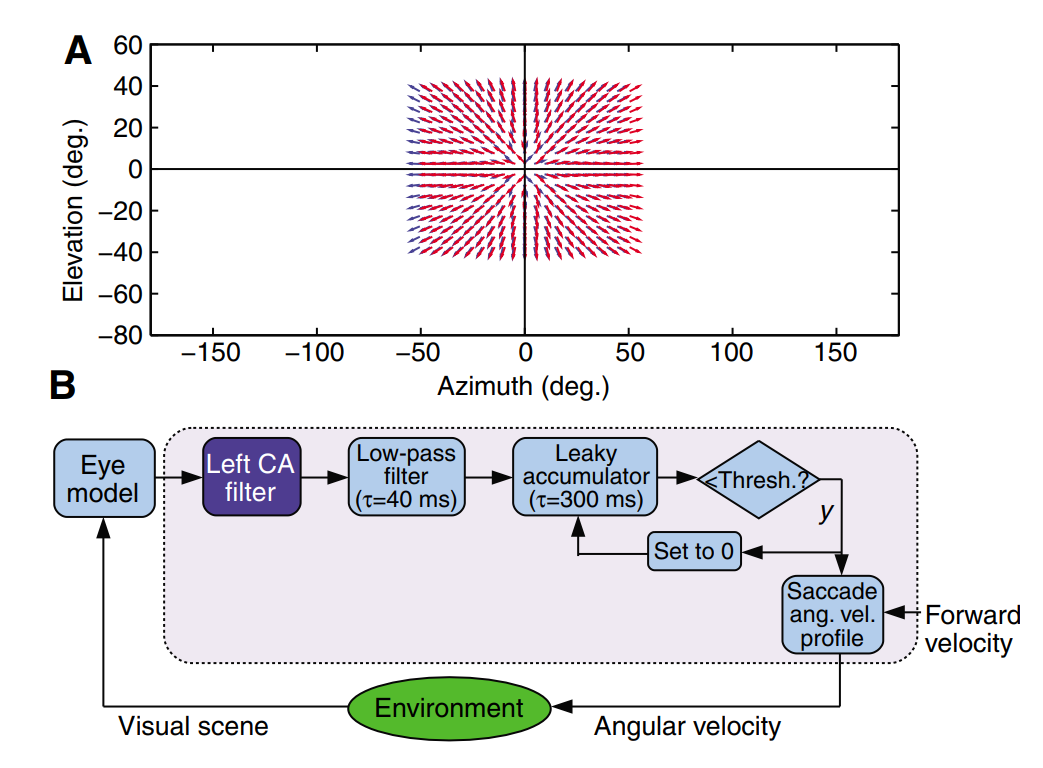
\includegraphics[width=0.9\textwidth]{Stewart2010CAModel}
  \caption{
    \label{fig:stewartca} The OF filter model: (Caption from \textit{Stewart et al.} Figure 7):
    Collision avoidance (CA). (A)The CA filters used in the
    model. Each covers ~105 deg. of azimuth but they are centred
    at $\pm 3$ deg. (elevation = 0 deg.). (B) Control diagram for collision
    avoidance. Only the half of the system that triggers rightward
    saccades is shown for clarity; the other half has an identical
    configuration. The dark blue box represents the blue wide-field
    filter in A. The reset operation also applies to the other half of
    the system, i.e. a saccade in one direction sets both
    accumulators to 0. Thresh., threshold; ang. vel., angular velocity.
  }
 
\end{figure}

\subsection{ The Mushroom Body for Visual Navigation } \label{MBBackground}
The Mushroom Body neuropils are structures present in the brains of all insects though they are
largest in the brains of hymenoptera. They are known to play a critical role in olfactory
learning, and have been thought to play a role in visual memory in hymenoptera since 1982
at the latest\cite{Mobbs1982}. In 2016 a Mushroom Body circuit was proposed by \textit{Ardin et al.}
to allow emulation of the structure in a simulated desert ant \cite{Ardin2016}. The simulated
ant's view is taken from 1cm above the ground and has a field of view of $296^{\circ}$ azimuth
by $76^{\circ}$ elevation. A ratio of $4^{\circ}/pixel$ is used to give a $19\times74$ pixel image.
This image is then downsampled to 10$\times$36 pixels to give a realistic resolution for ant vision.
A $1\times360$ vector is used for further processing.
\newline

The generalised MB circuit is a three layer neural network: The first layer consists of a set of
visual Projection Neurons (vPNs), these connect to the second layer of standard artificial neurons
referred to as Kenyon Cells (KCs), and finally these KCs connect to a set of Extrinsic Neurons (ENs).
The reader should note that any reference to the weight of a Kenyon Cell herein is specifically referring
to the weight of the connection between that KC and the Extrinsic Neuron; this abstraction is made for
ease of reference.
\newline

The model by \textit{Ardin et al.} (shown in Figure \ref{fig:ardinmb}) consisted of 350 vPNs
(one for each pixel in the downsampled image). In the second layer we have 20,000 KCs each of
which receives input from 10 randomly selected vPNs; each KC requires coincident input from multiple
vPNs to fire. Every KC is then connected to a single EN which sums the number of KCs which are
activated by the input image. The network is trained by providing a reward signal at regular
intervals. If KC activation coincides with a reward signal, the connection strength to the EN is
greatly reduced. The single EN simply gives a familiarity measure for the image seen. The agent
decides on its next action by scanning to find the direction of greatest familiarity.
\newline

\begin{figure}
  \centering
  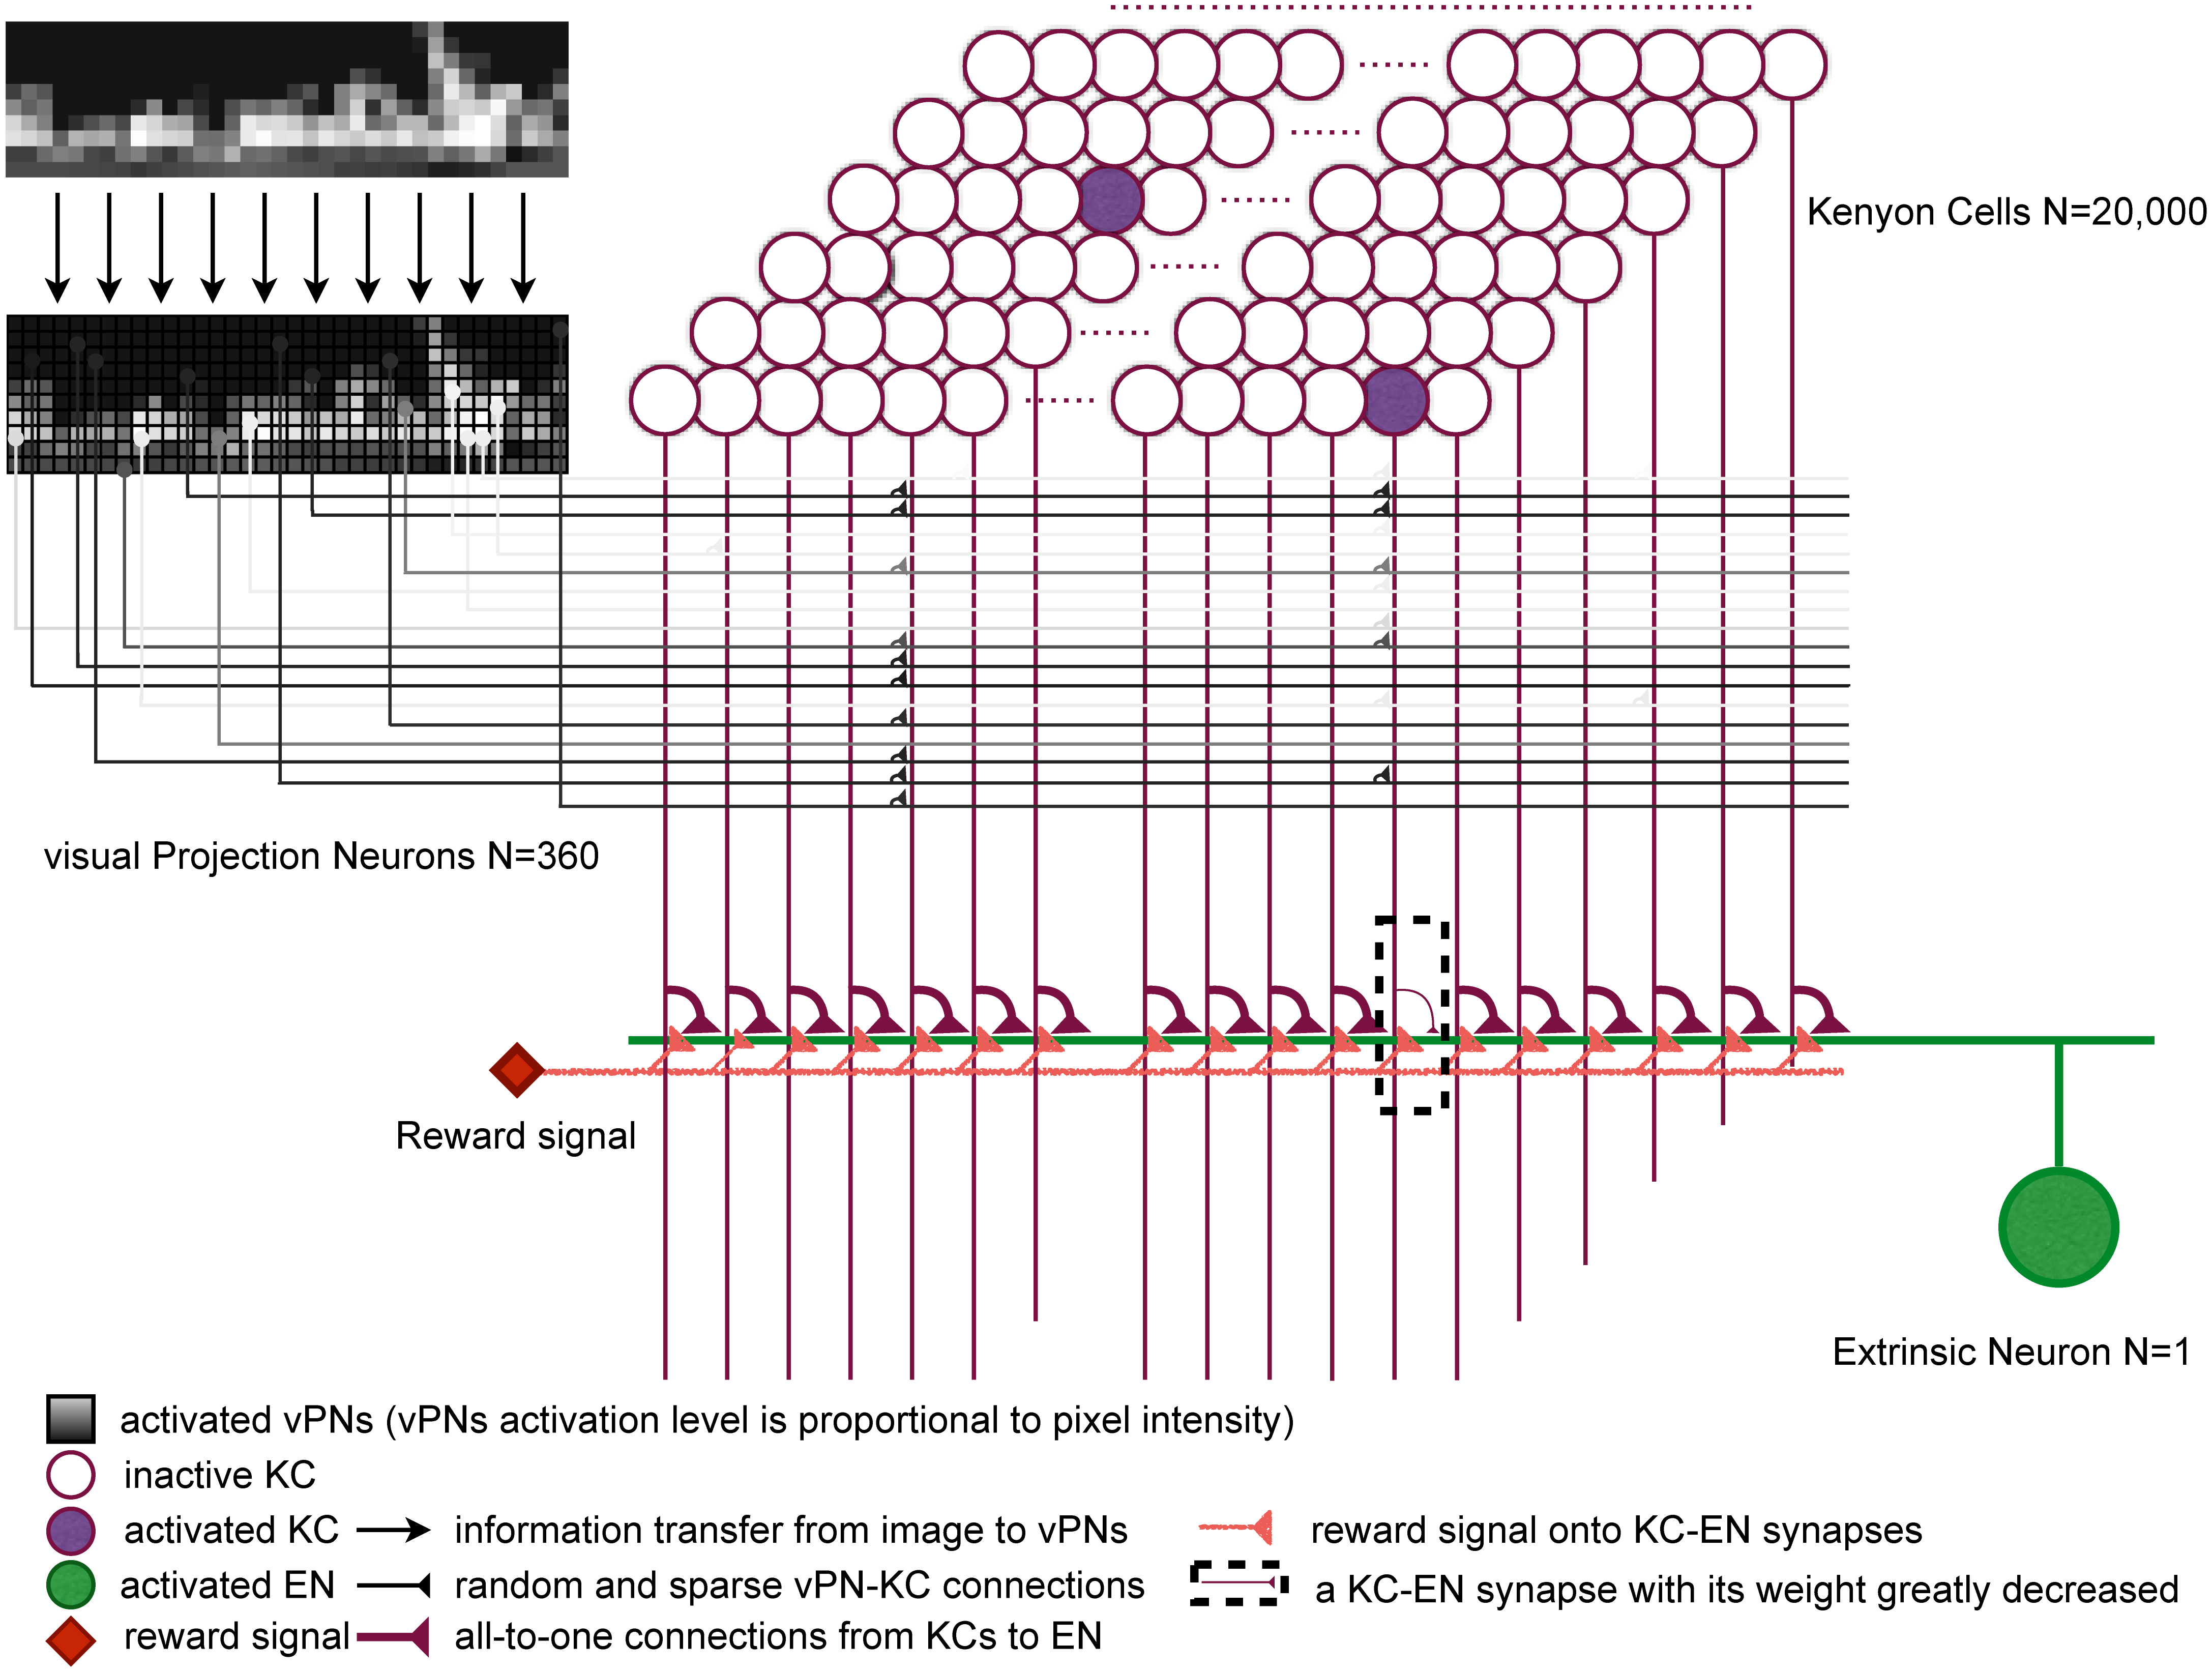
\includegraphics[width=0.9\textwidth]{Ardin2010MBModel}
  \caption{
    \label{fig:ardinmb} The Mushroom Body circuit: (Caption from \textit{Ardin et al.} Figure 2):
    Images (see Fig 1) activate the visual projection neurons (vPNs). Each Kenyon cell (KC) receives
    input from 10 (random) vPNs and exceeds firing threshold only for coincident activation from
    several vPNs, thus images are encoded as a sparse pattern of KC activation. All KCs converge on
    a single extrinsic neuron (EN) and if activation coincides with a reward signal, the connection
    strength is decreased. After training the EN output to previously rewarded (familiar) images is
    few or no spikes.
  }
\end{figure}

This version of the MB circuit has demonstrated the capacity to learn scene information, as well
as recapitulate routes by using the scanning technique \cite{Ardin2016}. In 2016, \textit{Eberding}
implemented the Willshaw Network (WN) on AntBot, which resembles the Mushroom Body neuropils (see \ref{sec:wn}); he
demonstrated that the network allowed the agent to perform visual navigation through a sparse testing
environment\cite{Eberding2016}. The agent navigates by scanning, computing unfamiliarity, and finally
choosing the direction of minimum unfamiliarity. In order to save on computational resources, the
KCs are binary rather than spiking (we hope to explore a spiking model in the future). While this does
generate a correct route, it is not as continuous as those performed by real ants.
\newline

In 2017, \textit{Zhang} implemented a route following strategy originally proposed by
\textit{Koszhabashev and Mangan} which employed klinokinesis in place of scanning. Klinokinesis
is one of two main forms of kinesis - the movement of an organism in response to stimulus - in which
the turning rate is proportional to stimulus intensity. In \cite{Zhang2017}, the
stimulus is given by the unfamiliarity metric generated by the MB model. The step size between each
turning point as well as the turning angle depends on the unfamiliarity of the current view. The same
algorithm from \cite{Kodzhabashev2015} is used to perform klinokinesis on the robot.
\newline

A separate model, also implemented by \textit{Zhang}, added seven extrinsic neurons. Each EN is then
used to represent one of eight directions relative to the robot's current heading; if we take 0$^\circ$
to be the robot's forward direction then the other seven directions correspond to $+45^\circ$,
$+90^\circ$, $+135^\circ$, $\pm180^\circ$, $-135^\circ$, $-90^\circ$, and $-45^\circ$. This model was implemented as a way of
combining the MB model for visual navigation and the CX model for path integration. While, path
integration and the CX model are not explored in this project, the model is still worth discussing,
as it may still be used to encode a desired response to specific stimuli.

% Should the Klinokinesis Algorithm be given here?

\subsection{The Willshaw Network} \label{sec:wn}
The Willshaw network is a specific style of neural network with an interesting background; capable of
instantaneous learning, high capacity, and importantly, resembling the structure of the Mushroom Body
inputs, storage layer, and outputs.
\newline

The idea behind the network stems from the effect of passing a pattern of light beams through two
patterned pinhole cards and a lens to create a pattern of refraction on a screen. The pattern output
on the screen is said to be a correlogram of the two patterns. Intuitively, the light pattern output
at $A$ can be passed through filter pattern $B$ to produce pattern $C$. This idea is then refined by
\textit{Willshaw et al.} into a simple, three-layer neural network. As an aside, though the terminology of artificial
neural networks is not used in the original paper, the model presented is designed to be interpreted as
a biological neural network, so interpretation as an ANN is a case of semantics. The three layers of the
Willshaw network are quite simple: a set of input neurons $N_B$ are represented as parallel horizontal
lines; a set of output neurons $N_A$ are represented as parallel vertical lines; and finally the storage
layer is a map of all of the intersections between the inputs and outputs. The storage layer is made up of
artificial synapses which are initially inactive (weight zero). The synapses are activated (weight set to one)
when the input pattern and output pattern activate the same synapse. More succinctly, synapse $c_{i,j}$ is set
to 1 when $a_i$ and $b_j$ are activated simultaneously.

\begin{figure}[h]
 
  \centering
  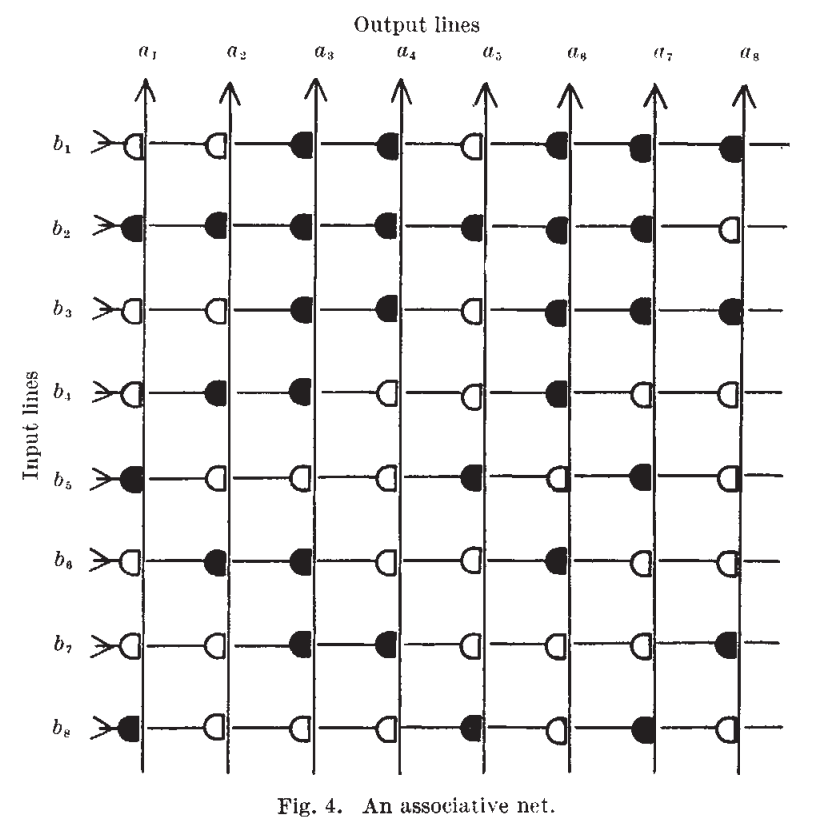
\includegraphics[width=0.5\textwidth]{Willshaw1969Model}
  \caption{
    \label{fig:willshawnet} The original network figure (Fig. 4) from \textit{Willshaw et al.} \cite{Willshaw1969}.
  }
 
\end{figure}

This style of network can be transformed into something which models the MB circuit presented by \cite{Ardin2016}.
The input neurons $N_b$ become the vPNs with multiple inputs going to each synapse. The synapses themselves become the
KCs, though the weighting convention is reversed with zero being active, and one being inactive. We reduce the set of
outputs $N_a$ to a single line which represents our reward signal. Coincidence of a pattern of KC activation and a reward
signal results in instant learning of that pattern by the learning rule set up in \cite{Willshaw1969},
just as in the MB circuit. Finally we must add the Extrinsic Neuron to
the model as there is no parallel in the original Willshaw Net. As before the EN simply sums the weights of the KCs activated
on presentation of an input pattern. Thus, the Willshaw net can be used to model the Mushroom Body circuit.
\newpage

%%%%%%%%%%%%%%%%%%%%%%%%%%%%%%%%%%%%%%%%%%%%%%%%%%%%%%%%%%%%%%%%%%%%%%%%%%%%%%% PLATFORM
\section{ Platform } \label{sec:platform}
In order to test the hypothesised models for ant navigation we use a simple robot autonomous - AntBot.
AntBot was originally developed by \textit{Eberding} in 2016; here we will discuss his design and
implementation, upon which we develop our algorithms.

\subsection{ Hardware }
AntBot's predecessor, Roboant, was originally designed by \textit{Kodzhabashev} \cite{Kodzhabashev2014}
as a compact Android robot. The robot required only four components: A sufficiently powerful Android
phone (A Google Nexus 5 was used) as the brain, the Zumo Robot shield by Pololu as the chassis,
an Arduino microcontroller to allow them to communicate, and finally a 360$^{\circ}$ camera attachment.
AntBot uses the same basic structure, however, a Dangu 5 Rover chassis is used as the base, and
therefore an alternate motor controller board had to be used.
\newline

The Android phone was chosen as the control module for the robot for a number of reasons. Firstly,
the hardware; a modern smartphone allows a compact, powerful platform on which to build the
software system as well as providing built in sensory systems and the libraries to use them (e.g. the
camera). The Google Nexus 5 is more than capable of running image processing software, analysing
optical flow patterns, and simulating the required artifical neural networks required for this project.
Using an Android platform also allows for modular software design (See section \ref{subsubsec:droid}).
In order to mimic the near 360$^{\circ}$ field of view (FOV) given by the ant's compound eyes, we use a
panoramic lense (the Kogeto Dot), which uses a convex mirror to give a full 360$^{\circ}$ FOV. This
lense is attached to the front camera and requires some pre-processing to retrieve the desired
$360\times40$ image. As with Roboant, the Android phone is connected to an Arduino using a serial
interface. Commands are sent from the phone to the Arduino which then executes the relevant commands
on the motor board to provide motion control.

\begin{figure}[t!]
  \centering
  \begin{minipage}[t!]{0.45\textwidth}
    \centering
    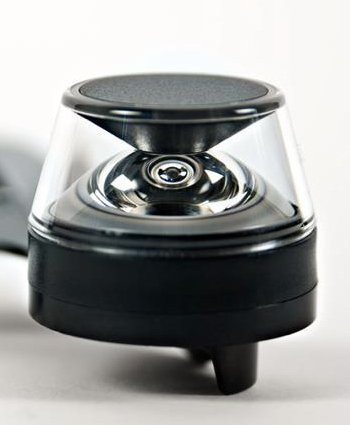
\includegraphics[width=0.9\textwidth]{KogetoDot}
    \caption{The Kogeto Dot 360$^\circ$ panoramic lens.}
  \end{minipage}
  \hfill
  \begin{minipage}[t!]{0.45\textwidth}
    \centering
    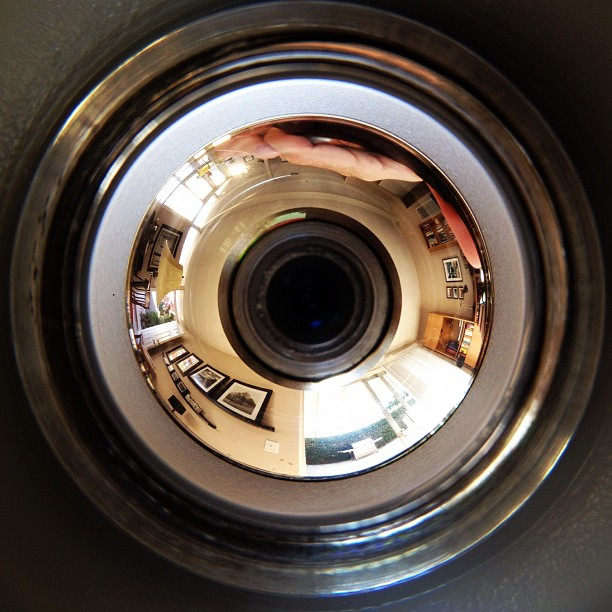
\includegraphics[width=0.9\textwidth]{PanoramicView}
    \caption{A sample of the view given by the lense before any processing.}
  \end{minipage}

\end{figure}

\subsection{ Software }
\subsubsection{ Android } \label{subsubsec:droid}
The architecture of the Anrdoid operating system is such that applications can (subject to certain
constraints) run in parallel while broadcasting important information to one another. This allows
for a modular, ROS-like\footnote{Robot Operating System - ROS: http://www.ros.org/}
system in which we can have a dedicated application for each navigational subsystem employed by AntBot.
\newline

In this fashion, \textit{Eberding} implemented an Android Application Network (AAN) consisting of
five applications:
\newline

\begin{enumerate}
\item{
    The \textit{AntEye} application - This application is the main application in the network and
    provides the user interface, along with all camera interaction and visual processing. To summarise;
    the visual processing system takes the 360$^{\circ}$ panoramic image from the camera, extracts
    the blue channel information, crops out the ring which contains the actual image and reshapes
    this into a $360\times40px$ image, and finally downsamples this to a $90\times10px$ image. This
    final image is then used by any application which requires visual information.
  }

\item{
    The \textit{Path Integration} application - This application is responsible for performing all
    tasks related to Path Integration (PI). PI is the process of computing displacement
    based on a series of consecutive moves. In \textit{Eberding's} original implementation this
    application did not perform PI, but was instead used as a utility application to record orientation
    and distance travelled. \textit{Scimeca} extended this application to implement PI, using both a
    mathematical and neural approach.
  }

\item{
    The \textit{Visual Navigation} application - Similar to the PI application, the VN application
    houses the necessary components for performing visual navigation tasks. \textit{Eberding}
    implemented both the Willshaw (Mushroom Body) network, and also a Perfect Memory (PM) module both
    of which were extended by \textit{Zhang}. There also exists a super-class for visual navigation
    algorithms.
    }

\item{
    The \textit{Combiner} application - This application is used to combine the output from the

    VN and PI applications in order to compute what action the robot should take. This application
    governs the movement of the robot based on the two primary navigational systems.
  }

\item{
    The \textit{Serial Communications} application - This application governs all communication from
    the Android phone to the Arduino and server-interface. Android forbids multiple applications from
    using a single serial or Wifi port, so this application was developed as an intermediary to allow
    the other applications in the network to communicate through a single application.
    }
\end{enumerate}


\textit{Eberding's} implementation included a server interface which was used to control the robot
remotely
using the phone's Wifi hotspot and Serial Communicatin App, however, this interface has not been used
since the original implementation. For more information, please see \cite{Eberding2016}. It should
also be noted that, due to work conducted during previous iterations of this project, it may not
be possible to follow this exact structure.


\subsubsection{Arduino}
The Arduino software can be split into two sections: the \textit{parser} and the \textit{executioner}.
The parser will receive commands from the serial port and convert them into a series of movement
commands. These movement commands are then sent to the motor board by the executioner. Encoder
information may be gathered by the Arduino and sent back to the phone for processing.
For this project,
the Arduino code has not been modified. We only required the use of two commands for this project;
\textit{go}, which allows the robot to move indefinitely at a set speed, and \textit{turn}, which
allows the robot to turn to a desired (relative) angle. The \textit{go} command also allows the
operator to specify a speed for the left and right sides allowing the robot to move in smooth arcs.
A full list of commands can be seen in Table \ref{tab:commands}.

\begin{center}
  \begin{table}
    \begin{tabular}{ | l | l | p{7cm} | }

      \hline
      \textbf{Command} & \textbf{Message} & \textbf{Action} \\ \hline
      
      Heartbeat & x \textit{seconds} n &   Feedback sent to verify a stable connection between the
                                           phone and the Arduino. A signal is sent every second with a
                                           timestamp and checked. \\ \hline

      Move & t 0 \textit{distance} n & Travel a set distance in metres. \\  \hline
      Turn & t 0 \textit{angle} m 0 n & Turn a set angle (in degrees). \\ \hline
      Turn and Move & t \textit{angle} m \textit{distance} n & Turn by a specified angle then move the
                                                               specified distance. \\ \hline
      Turn left & \textit{l} & Turn left indefinitely. \\ \hline
      Turn right & \textit{r} & Turn right indefinitely. \\ \hline
      Halt & \textit{h} & Stop any command in progress and stop the robot. \\ \hline
      Go & g \textit{leftSpeed} \textit{rightSpeed} n & Move indefinitely with specified left and
                                                        right speeds. \\ \hline
                               
      
      \hline
      


      
    \end{tabular}
    \caption{The available commands on the Arduino and the messages sent to invoke them. Those
      values which are changeable are shown in italics. The \textit{go} command was added by
      \textit{Scimeca}. This table was adapted from \cite{Eberding2016, Scimeca2017}.
    }
    \label{tab:commands}
  \end{table}
\end{center}

Previous works have mentioned a message of the format \textit{e e1 e2 e3 e4} n. This message was used
to send wheel encoder information from the Arduino to the phone, however, this message was only sent
during the execution of a particular function and it has since been removed from the Arduino code.
There are currently no utilities available to retrieve and reset encoder values on-demand from the
phone, though such utilities should not be difficult to implement.

\subsection{Modifications}
Some hardware modifications have been made to the robot. Upon the uptake of this project, AntBot
was powered by six 1.2V AA NiMH batteries wired in series (using a simple power pack). This power
pack was connected to the motor board (and subsequently the motors) by a pair of 9V connectors. The robot
had to be opened up in order to connect or disconnect the batteries from the motors. The batteries themselves
had to be extracted from the power pack and charged individually. These actions, repeated often by the current
project and predecessors had caused wear on the power pack and the internal wiring. The wires themselves
needed re-soldered multiple times. In order to have a more robust platform for testing, the on-board
power system was modified. The aim of the modification was to add a power source which could be charged in-place.
As such a new power source which could be charged as required without removal was added, along with external
charging ports and a switch. The internal wiring was re-done such that power could either flow from the
external ports to the battery, or from the battery to the motors controlled by the external switch. The new
power source is a 9.6V NiMH power pack. Motor speeds and systems which depended on them required re-tuning
after completion of the modifications. The required modifications to chassis (holes drilled for components)
were done by the Informatics workshop. The wiring, research and sourcing of parts were performed as part
of the project.
\newpage

%%%%%%%%%%%%%%%%%%%%%%%%%%%%%%%%%%%%%%%%%%%%%%%%%%%%%%%%%%%%%%%%%%%%%%%%%%%%%%% METHODS
\section{ Methods } \label{sec:methods}
\subsection{Optical flow models for Collision Avoidance}
\subsubsection{Time-to-Collision}
We attempted to follow the outline presented by \textit{Low and Wyeth} as, at first glance, it seems
a straightforward and neat solution. However, this method of computation for the TTC relies on the
assumption that the camera view only ever moves in the forward direction which is not appropriate
for AntBot (See Section \ref{sec:platform}). So we look instead at the paper by \textit{Souhila and Karim}
for an alternative; for this method, we must compute the \textit{focus of expansion} or FOE, however,
their method of computing the FOE again relied on forward motion of the camera and did not translate
well into AntBot. A more general method for computing the FOE is given by \cite{ODonovan2005}:

%Copy of description from old backround so I don't have to type out the maths again.
%\textit{Included for skeleton purposes.}
%However, this method of computation relies on the assumption that the robot only ever moves in the
%forward camera direction which is not appropriate for AntBot (See section \ref{sec:platform}).
%We must look for an alternate way to compute TTC. Fortuntely, such information is easily
%computable from the \textit{focus of expansion} (FOE), the point from which all flow vectors
%originate.
%\newline

%A general method for computing the FOE is given by \cite{ODonovan2005}:

\begin{equation}
  FOE = (A^TA)^{-1}A^T\mathbf{b}
\end{equation}

\begin{equation*}
  \begin{split}
 A = 
\begin{bmatrix}
  a_{00} & a_{01}\\
  \dots  & \dots \\
  a_{n0} &  a_{n1}
\end{bmatrix}
\qquad
\end{split}
\begin{split}
\mathbf{b} =
\begin{bmatrix}
  b_0 \\
  \dots \\
  b_n
\end{bmatrix}
\end{split}
\end{equation*}
\newline

Where, for each pixel $p_i = (x, y)$, the associated flow vector is given by $\mathbf{v} = (u, v)$.
We then set $a_{i0} = u, a_{i1} = v$ and finally $b_i = xv - yu$. The TTC can then be computed as:

\begin{equation}
  TTC = \frac{d}{v} = \frac{y}{\frac{\partial y}{\partial t}}
\end{equation}

Where $y$ is the vertical distance of some point $p = (x,y,z)$ from the
FOE, $\frac{\partial y}{\partial t}$ is the velocity of translational motion of $y$, and
$d$ and $v$ are as given in (\ref{eqn:lowttc}).
A full derivation is given by \textit{O'Donovan} from whom we have adapted this equation.
\newline

Finally, we can simplify this to the desired equation from \cite{Souhila2007}:
\begin{equation}
TTC = \frac{\Delta_i}{|\vec{V}_t|} \dots
\end{equation}
Where $\Delta_i$ is the distance of a point $p_i = (x,y)$ from the FOE, and $|\vec{V}_t|$ is the
translational velocity of the camera computed from optical flow\cite{Souhila2007}. 
\newline
This time-to-contact is then appropriately thresholded and a reaction is generated based on the
position of the focus of expansion which provided a simple method of replicating the balance strategy
used by \cite{Souhila2007} as the FOE will be drawn to one side based on the motion parallax observed.
Initial instability in the computation of these properties was countered with by averaging the properties
across a series of frames to reduce potential noise.
\newline

The generated responses were to be halt on detection (for debugging purposes), and triggering of a
smooth turn away from the obstacle. This technique was designed to be used with a sparse optic flow
field, however, a version using a dense flow field was attempted. The computation across a dense
flow field was found to be impractical. No formal results have been collected using this system; any
apparant functionality was found to be luck instead of a working system. Analysis of functionality
of such a system on AntBot is left for Section \ref{sec:results}.


\subsubsection{Filtering}
Here a dense optical flow field is used, and in order to explain the filtering process, it is important
to discuss the flow computation itself. The optical flow is computed using openCV's
\textit{calcOpticalFlowFarneback()} function. When given two consecutive frames the function returns
a matrix $M$ of arrays of type double. $M_{y,x}$ is a one-dimensional array of length two which contains
the displacement in each axis of the respective pixel (i.e. $M_{y,x}[0]$ gives the displacement of the $x$
coordinate, and $M_{y,x}[1]$ gives the displacement of the $y$ coordinate.
\newline

An optical flow filter was previously implemented by \textit{Scimeca} for the purpose of speed retrieval. 
As collision avoidance in optical flow relies on detecting a difference in motion between two sides
the same filtering method could be re-purposed for collision avoidance. Though inspired by \cite{Stewart2010},
our method for performing the computation and avoidance was modified slightly for the sake of
implementation on AntBot. Instead of creating
a left and right filter, we create left and right flow frames by taking rotating the image frame
by a certain angle left or right as in \cite{Scimeca2017}. However, we reduce the angle from $\pm 45^{\circ}$
\cite{Scimeca2017} to $\pm 16^{\circ}$. It was found that the size of this angle had a mild effect on the region of the 
image which would trigger responses; a larger angle would result in higher sensitivity to the sides of the
robot, a smaller angle results in higher frontal sensitivity which was desired for the CA system. We only
want the robot to avoid obstacles to the front, obstacles to the sides should not trigger responses. The offset
angle was tuned manually and $\pm 16^{\circ}$ was found to perform well; smaller angles resulted in
an insensitive system, and larger resulted in more noise, though performance was still good. The filter
itself is the same as the second filter from \cite{Scimeca2017} which was already implemented on the robot.
\newline

The filter is constructed as an $Nx3$ matrix $F$ such that:

\begin{equation}
F_i = [ \quad sin(-\pi + i\frac{2\pi}{N}) \qquad 0 \qquad 0 \quad ] \quad \textit{for} \quad i \in \{0, N - 1\}
\end{equation}

where $F_i$ is the $ith$ row of $F$. Intuitively each row corresponds to a pixel value in the $x$ axis.
\newline

Once the filter is computed, we retrieve the flow for each pixel by adding the displacements
retrieved from \textit{calcOpticalFlowFarneback()} to the pixel value. 
For each value of $x$ we apply an offset of $\pm 4px$ which corresponds to our left and right frames centred at
$\pm 16^{\circ}$. For the $ith$ pixel, with filter vector $\bar F_i$ and flow vector  e$\bar O_i$ we apply the filter
simply by computing the projection:

\begin{equation}
  P_i = \bar F_i \cdot \bar O_i
\end{equation}

This allows us to measure the geometric difference between the expected and actual pixel motion. The computation
for a single frame simply sums all of these projections:

\begin{equation}
  FlowSum = \sum_{i = 0}^{K - 1} P_i
\end{equation}

where $K$ is the number of pixels in the image, in our case $K = 900$. This sum is computed for both shifted frames
and a tuning factor is applied for the simple purpose of making the numbers returned easier to handle.
\newline

Now we have defined a way of computing speed differences between the two sides, we
can start to define behaviour. In the case an obstacle is seen on one side of the image, we expect the speed
on that side to be higher due to motion paralax. Thus, we simply compute the difference between the
two sums:

\begin{equation}
FlowDifference = LeftFlowSum - RightFlowSum
\end{equation}

which gives us our final stimulus to be used to generate a reaction. Here we employ the idea of ``leaky'' accumulators
from \cite{Stewart2010}. An accumulator is kept for both sides of the frame. The raw difference is thresholded to account
for noise such that only significantly positive or negative values contribute to behaviour; this is known as the
\textit{accumulation threshold}. Once the accumulator on one side exceeds its \textit{reaction threshold}, an immediate
turn away from the perceived obstacle will be performed. The turn is simply a $\pm 20^{\circ}$ rotation using the robot's
\textit{turnAround()} function. The accumulators are reset periodically to avoid a build up of old flow information.
A separate method of accumulation was trialled out of interest whereby a single accumulator would be fed the raw difference
and a sufficiently large positive or negative value would trigger the appropriate response. No difference was noticed in
performance and so separate accumulators were kept. While this implementation was simple, and not as refined
as we would have liked, it did demonstrate impressive performance in navigating arenas of varying density.

\subsection{The Mushroom Body}
This section will be less of a formal declaration of method, and more a discussion of the process undertaken to get
the Mushroom Body circuit working in a robust manner.

The Mushroom Body circuit (implemented as a Willshaw Net) was originally implemented by \textit{Eberding} when he
initially developed the platform. Though the implementation does mirror the model of \textit{Ardin et al.}, the model
struggled to perform to the same degree despite potentially having more visual information due to the higher resolution
image of AntBot. The nature of our experimental scenario required (at least initially) that a scanning behaviour be used
to perform visual navigation and this is the context in which we shall frame our discussion; this because \textit{Zhang}
did manage to achieve significantly improved results using Klinokinesis as a route following strategy. Initial attempts
at scanning resulted in extremely poor performance with seemingly no capacity for memory present in the network beyond
blind luck. The first and most obvious issue was the scanning behaviour itself; while the robot was to turn through a
$60^{\circ}$ arc in increments of $6^{\circ}$, the actual arc was far larger ($> 100^{\circ}$). On closer inspection of the
control code on the Arduino, the problem could be seen as the control method. The turning command relies on a calculation
based on encoder clicks per degree; while simple and appropriate for general use, this style of control generally struggles
to make precise movements, such as scanning increments.
\newline

To remedy this, we opt for a different style of scanning which
we will refer to as \textit{visual scanning}. Since AntBot has a $360^{\circ}$ view, we instead take a still image, and rotate
it, showing each rotated frame to the network and receiving a familiarity measure; this change was felt justified as we are
concerned with the performance of the MB model and did not wish to be hampered by robot control issues (though these issues
can, and we feel should be fixed if possible - See Section \ref{sec:discussion}). These values are stored in an array (as
with standard scanning), the minimum value is selected and the angle computed by taking the distance from the centre-point
of the array and multiplying by the number of pixels traversed horizontally then multiplying again by the constant $4$ (degrees/pixel).
In the first iteration, a highly granular scan was used, however, this was found to be less effective and more prone to erroneous
familiarity measures. Reducing the number of image angles while scanning over the same arc resulted in more stable performance. In total
$17$ different angles (from $-16px$ to $+16px$ in increments of $2px$) are compared. The image rotation itself is done with
a basic array rotation algorithm which manipulates matrix columns. With the visual scanning, the problem of robot
control was largely eliminated. 
\newline

However, a common behaviour was still observed. Be it physical or visual scanning, the robot always performed a turn in the same direction,
at the same angle (i.e. the most familiar direction was always to the extreme left). For the purposes of debugging and visualising the
network and its outputs a two-part tool \textit{AntBotStats} was developed (see Section \ref{sec:abs}). Visualising the output of the
network showed that the returned familiarity was not following the correct pattern over a scan.


\begin{figure}
  \centering
  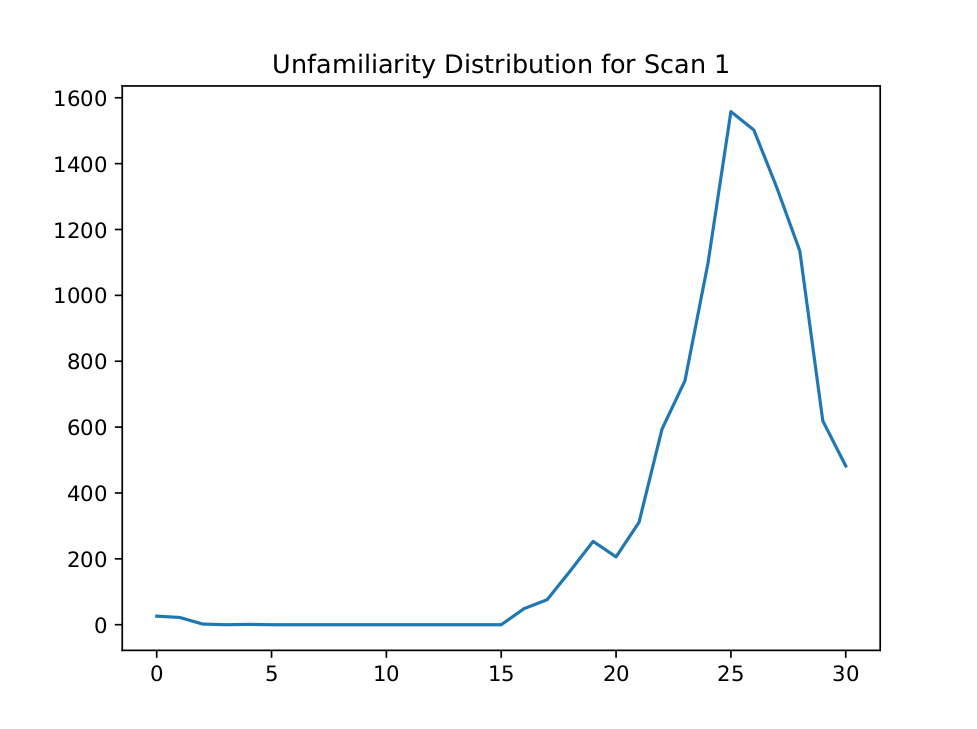
\includegraphics[width=0.7\textwidth]{MB-Bad-Familiarity}
  \caption{
    \label{fig:mbbad} The erroneous familiarity pattern displayed by the network. The plot shows the
    familiarity response of the Extrinsic Neuron (y-axis) against the index of the scan (x-axis). 0
    denotes the leftmost direction, 15 directly ahead, and 30 the rightmost direction. This was a simple
    plot produced early in the debugging process, hence the lack of axis labelling and higher number
    of scan points. 
  }
\end{figure}

\begin{figure}
  \centering
  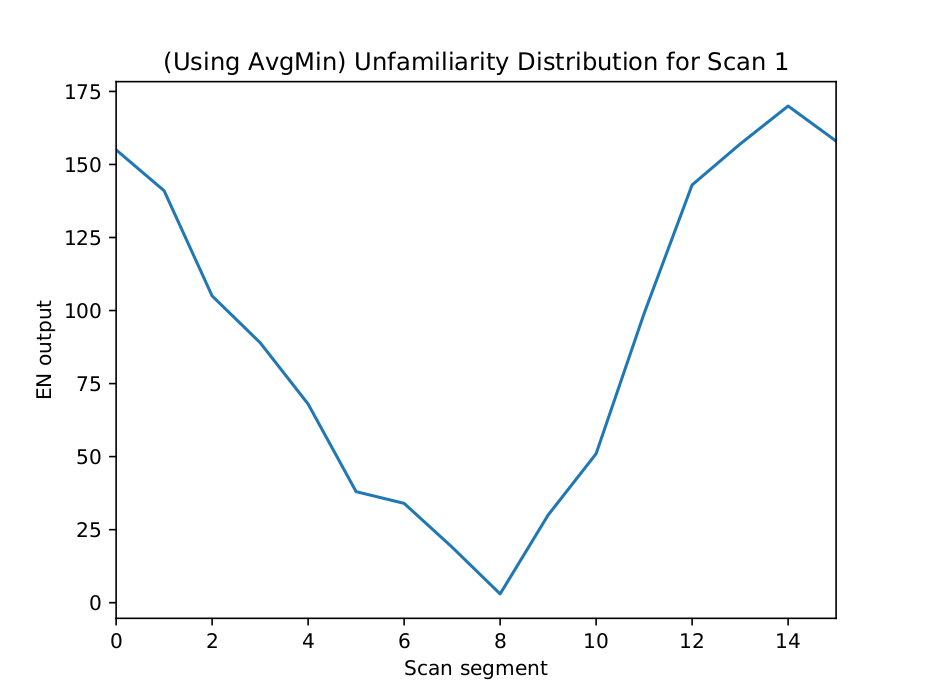
\includegraphics[width=0.7\textwidth]{MB-Good-Familiarity}
  \caption{
    \label{fig:mbgood} The expected familiarity response of the Extrinsic Neuron. Note the improved
    range of the response along with the clearly defined minimum.
  }
\end{figure}

In figures \ref{fig:mbbad} and \ref{fig:mbgood} (both produced using visual scanning) we see that the pattern being
returned by the early network with scanning was far from what it should have been. The EN response of 0 should, in theory,
correspond to the most familiar angle. Figure \ref{fig:mbbad} clearly shows that there is a problem with the Kenyon Cell
activation in the network; a presented image should activate somewhere in the range of 200 to 500 KCs (this is rough due
to the pseudo random construction of the network). The EN response shows that at least $1000$ KCs were activated by some
scan angles; in almost all cases, an EN response of $0$ was caused by a lack of any KC activation (the familiarity measure
was initialised as $0$ in the network). To, fix this upper and lower thresholds on KC activation were added to the
network. If KC activation lay outside these bounds a \textit{maximum unfamiliarity} measure was returned; this value
was defined as the maximum number of KCs activated by an image during the learning process. The justification for introducing
bounds on KC activation was that too few KCs did not give enough information, while too many represented noise in the network.
Regardless of the justifiability of this decision, \textit{Ardin et al.} did not encounter such problems in their functionally
identical model.
\newline

It is here we must note again, \textit{Zhang's} improved performance using Klinokinesis; this suggests that the network itself
is likely not the issue. Upon performing further debugging
the problem revealed itself to be related to the visual scanning (just as the original scanning method had experienced similar
problems); due to a quirk of OpenCV in Java, the \textit{Mat} (matrix) objects are passed by reference (despite there being
no explicit instruction to do so, and no clear mention of such behaviour in the documentation). When Mat objects are passed,
a separate object called the \textit{matrix header} is actually passed which performs the same function as a pointer in a C-style
language. Thus, the image rotation algorithm was working correctly, but the image was being rotated in unexpected ways. Simply,
creating a copy of the Mat object inside the rotation function fixed the issue and the network began functioning correctly.
\newline

The final model is largely the same as in \cite{Eberding}; the only real modification being the Kenyon Cell thresholding.
Normalisation of the PN input was implemented but not found to make a noticable difference so raw PN values were used
to reduce complexity in the model. 


\subsection{AntBotStats}\label{sec:abs}
To aid in debugging the Visual Navigation system and production of results a two-part tool, \textit{AntBotStats} was developed.
The tool consists of an on-board Java class, \textit{StatFileUtils} (adapted from \textit{LogToFileUtils} \cite{Zhang2017} and a
Python parsing and plotting tool. The \textit{StatFileUtils} class is designed in such a way that title, plot type, and data can be
specified. The Python system then reads the file, produces the correct plots and outputs them to a PDF for viewing as a collection.
The tool is currently quite basic but is designed to be easily extensible to produce different information; for example a module was
added to produce trajectory plots from the Vicon motion capture system. 
\newpage

\section{Experimentation}\label{sec:test}
\subsection{General}
An experimental arena was constructed on the old Robocup practice pitch in G.17 in the Informatics Forum. This space was chosen
for its suitable size, locality, and easy access to recording equipment for Visual Navigation experiments. An enclosure was constructed
using old (mostly) preconstructed perimeter perimeter sections from the Robocup pitch which could be easily set up and dismantled as the
space was shared. The enclosure was added to act as a visual blind (Figure \ref{fig:arena}) in an attempt to reduce the background noise observed by the robot and
also to keep the distances on either side reasonable as it was noted by \cite{Scimeca2017} (and experienced first hand) that large differences
in distance on either side of the robot could cause drastic differences in the speed observed by the optical flow which would affect our
experiments. The perimeter blind was aligned with the tape markings of the football pitch to establish consistency.
\newline


\begin{figure}
  \centering
  \includegraphics[width=0.7\textwidth]{The-Arena}
  \caption{
    \label{fig:arena} The empty experimental arena.
  }
\end{figure}

As obstacles, early tests involved the use of large, obvious objects such as cardboard boxes. To try and create a more realistic
picture for AntBot, simple synthetic tussocks were constructed. These were constructed by taking $1m^2$ synthetic hedge wall panels and
cutting them down to different sizes. These were then fitted to rough-cut (in an effort to keep sizes non-uniform and somewhat
natural) wood blocks. The wood blocks compensate for the distance from the ground to AntBot's view height such that AntBot can only
see the synthetic plant (Figure \ref{fig:tussock}).
\newline

\begin{figure}[h]
  \centering
  \includegraphics[width=0.7\textwidth]{Tussock}
  \caption{
    \label{fig:tussock} An example of the tussocks used during experiments.
  }
\end{figure}

\subsection{Collision Avoidance}
Collision avoidance experiments aimed to test the basic functionality of the system; once demonstrated, we then wished to demonstrate
the robustness of the system. Finally, some experiments were performed out of sheer curiosity to determine how predictable the
system was and how well it coped with less random patterns of obstacles as well as determining the effect of different tuning modifications.
Each of the main experiments took place in a set arena and consisted of five runs to observe the consistency in performance. 
\newline

We start by demonstrating the basic functionality of the system using a series of three basic arenas: An empty arena, a single large obstacle
(a cardboard box present in the lab), and finally basic tussock interaction to ensure that the robot could detect and react to the synthetic
tussocks.

\begin{figure}[h]
  \centering
  \includegraphics[width=0.7\textwidth]{Tussock-Interaction}
  \caption{
    \label{fig:tussock} The arena used for basic tussock interaction
  }
\end{figure}

Once basic functionality is established, we then partition the arena into quadrants and start to increase tussock density per quadrant.
Starting with a density of $1/\textit{quadrant}$ the tussocks were placed randomly, as density increased tussocks were placed more
deliberately to attempt to block paths the robot had used previously (while still permitting enough space for the robot to navigate
through the environmnent). For these experiments in increasing complexity, the robot was always started from the South West corner
of the arena so that, regardless of the arena set up, the robot would have to perform some collision avoidance movements. The reader
should note that the initial tussock in the South East corner was a little more limited in where it could be placed. If placed too
far to the North, the avoidance turn triggered would turn the robot away from the arena; while this is technically successful as the
robot avoided the obstacle, the run would provide no useful data as the robot had not attempted to navigate the more complex arena; thus
the tussock in question was placed in a location that would trigger an inward turn. Each run was assessed on three criteria: Number of collisions,
Number of failed avoids, and whether or not there was a \textit{risk-on-end}. A collision was a direct impact with an obstacle that
should have been avoided where no turn was triggered in response (or the turn only occured after the collision). A failed avoid occurred in
the case where the robot did react but it was too late in doing so, or the robot could not turn enough due to space constraints. The
risk-on-end occurs when the robot is about to have a collision and the timer runs out (i.e. a collision would have occured in any other
navigational scenario); these occurred frequently, however, the vast majority of them would involve a collision with the side of the arena.
\newline

The final series of tests for the CA system involved setting up pre-determined arenas to see if the robot would respond in a predictable
fashion when presented with a particular pattern of obstacles. Some arenas were designed to test tuning parameters on the robot, for example,
to test how speed of the robot affects the reaction time and sensitivity of the system. These experiments presented largely unexpected though
useful and thought-provoking results.
\newline

\subsection{Visual Navigation}
Visual navigation experiments were conducted again across different arenas. These arenas were designed in such a way that the optical
flow would have little difficulty navigating them, while still providing enough visual information as to make the images captured
meaningful. A major failure in the collision avoidance system would result in a full reset (though minor failures were permitted to
continue). Each arena hosted two runs, one starting from the South West corner of the arena, the second starting from the South end
in the centre of the arena. A learning run was conducted using only the collision avoidance system to navigate through the arena
for 30 seconds. Image learning was not performed at any set intervals; a reward signal was sent once per main loop iteration \textit{if}
the new frame was available from pre-processing (synchronisation between threads means this may not always be the case). Upon finishing
the learning run, the robot was placed at the start point for the run.
\newline

The robot then attempts to recall the route using only visual memory. Scans were performed at regular time intervals, or if the robot
encountered an obstacle during a routine forward motion. The memory run had a time limit of 60 seconds, the extra time to allow for
scanning and decision making. If the robot reached the end of the route before the time was up it would behave
unpredictably as one might expect.
\newline

Eighteen experiments were run in total; the first eight were run as described above, the robot's behaviour was modified slightly
for the remaining ten. For the last experiments, the reward signal frequency was increased in an attempt to gain more information
about a route; in the first bout of tests, the reward signal was being sent approximately seven times per run, in the second bout
this was tripled, however, some stored images may overlap. The CA behaviour was also modified to allow the robot to stop before
turning instead of performing an immediate turn.
\newline

The routes were captured using the Vicon motion capture system; separate recordings were taken for learning and memory runs, the
files exported in .csv format then parsed and plotted using a module in \textit{AntBotStats}. All plots were set to the same scale
so as to allow direct comparison between results without needing to account for scale. Figures \ref{fig:autoscalerun} and \ref{fig:setscalerun}
suitably demonstrate this; though run MAB-5-2 was a success, the plot shown in Figure \ref{fig:autoscalerun} does not make this clear.

\begin{figure}
  \centering
  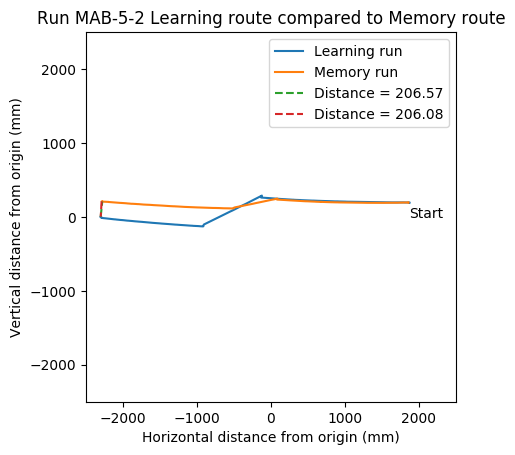
\includegraphics[width=0.9\textwidth]{MAB-5-2}
  \caption{
   \label{fig:autoscalerun}The autoscaled plot for run MAB-5-2.
  }
\end{figure}

\begin{figure}
  \centering
  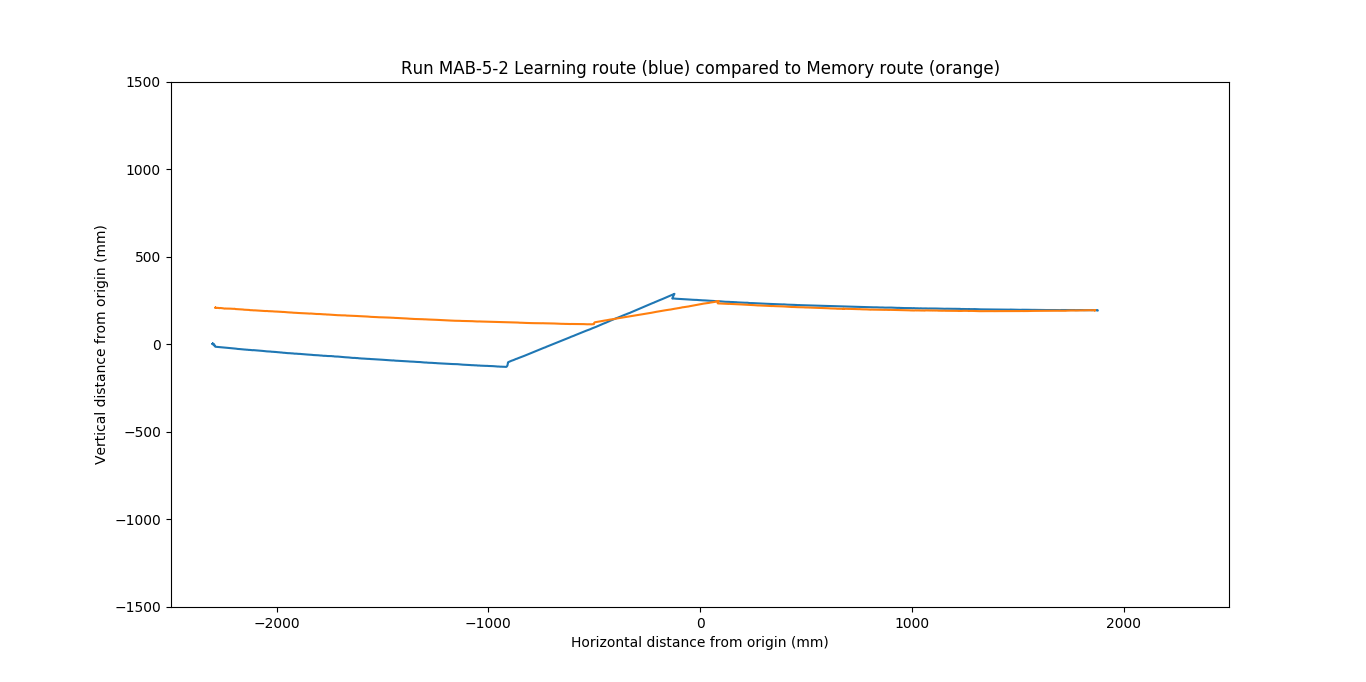
\includegraphics[width=0.9\textwidth]{MAB-5-2-S}
  \caption{\label{fig:setscalerun}The set-scale plot for run MAB-5-2; forcing the axes to a uniform scale over all runs gives a more accurate immediate
      view of the runs and their similarity.}
\end{figure}

\newpage

\section{ Results and Evaluation } \label{sec:results}
\subsection{Collision Avoidance}
\subsubsection{Time-to-Collision}
The TTC system was implemented with both flow field types; quite simply, performing the computation on a dense flow
field resulted in drastic reduction on speed and accuracy. We will discuss in the context of a sparse flow field. The
sparse optic flow field is computed using the \textit{Lucas-Kanade} method on the points returned by OpenCV's
\textit{goodFeaturesToTrack()} function. This function returns a Mat object which indicates the strong corners in an image.
In essence, it locates prominent features in the image which can provide consistent information. Inconsistensies
were noticed in the computation of the FOE and the speed (and hence the TTC) and many \textit{dirty} fixes were required to get the computation
functional. For a straightforward matrix calculation, this should not be the case. As the entire method was dependent on
the output of \textit{goodFeaturesToTrack()}, we felt it appropriate to check that the values being returned here were in-fact
reliable.

\begin{figure}
  \centering
  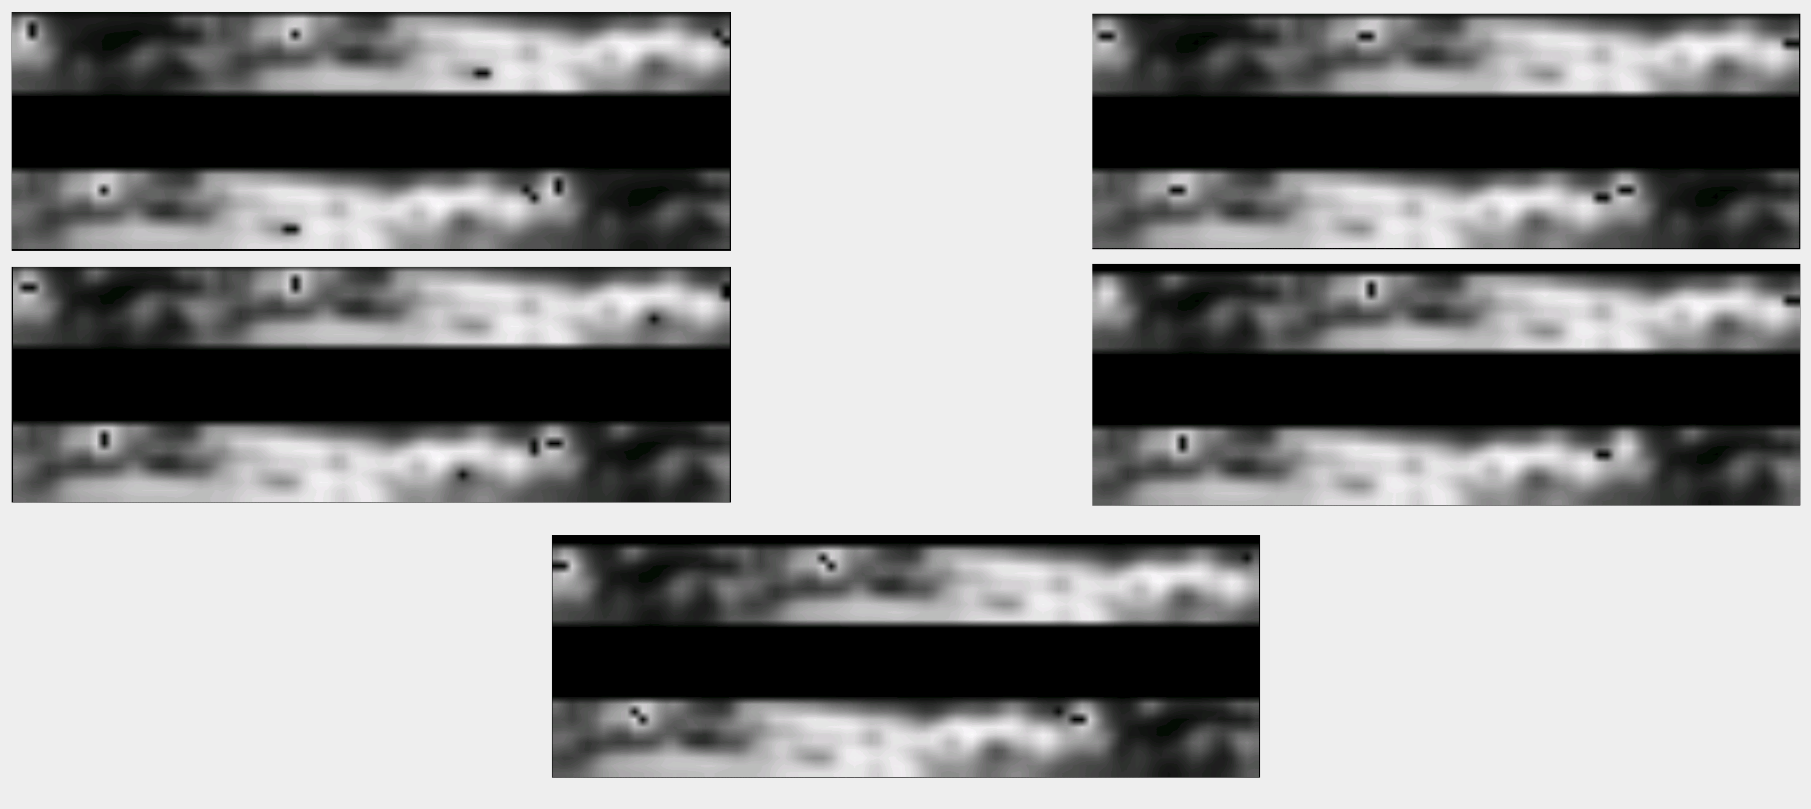
\includegraphics[width=0.7\textwidth]{OpticalFlowInconsistencies}
  \caption{
    \label{fig:ofbad} $\pm 45^{\circ}$ offset image frames showing the flow vectors computed at each point (distinct black
    pixels). The five images were taken over the course of one minute while the robot was stationary in G.17.
  }
\end{figure}

The flow vectors detected using the points returned by \textit{goodFeaturesToTrack()} can be seen in Figure \ref{fig:ofbad}.
Though the changes are not drastic, it can be seen firstly that varying motion is being detected in the image where none
exists though this \textit{noise} can be expected somewhat. Secondly, it should be noted that the different frames show different numbers
of features. While sat still, the algorithm cannot reliably detect consistent corners in the image. While the slight
differences in flow are not of major consequence, the different feature count was found to have a large effect
on the consistency of the computation as, every other frame, we are considering new information, and perhaps missing information
we had previously.
\newline

This flow information is key to computing both the speed of motion and the focus of expansion of the flow field; thus, the
time-to-contact is not accurate nor consistent. Though TTC was abandoned as a method for collision avoidance as part of this
project, there are a number of modifications that could be applied to make this more stable, however, any method of computing the
TTC relies on an accurate speed calculation. The works on which we based this system use encoder information to compute the
speeds, and while this is not entirely implausible from a biological standpoint \textit{[NOTE: STEPCOUNTING REFERENCE]}, we are currently
reliant on optical flow alone for speed retrieval. 

\subsubsection{Filtering}
The filtering system proved to be quite robust in its operation; over the thirty functional performance runs we only note four direct
collisions (complete failures of the system), and six partial collisions (the robot corrected but did so too late, or knocked a
tussock on the way past). The full set of results for the functional performance experiments are shown in Table \ref{tab:ofres}.

\begin{center}
  \begin{table}
    \begin{tabular}{|l|l|l|l|l|l|l|l|l|l|}
      \hline
      \multicolumn{4}{|l|}{\textbf{Optical Flow Functional Performance} }   &                  &              &               \\ \hline
                   & \textbf{Arena 1} & Empty              &             & \textbf{Arena 2} & Single Box   &               \\ \hline
      \textbf{Run} & Collision        & Failed avoid       & Risk on end & Collision        & Failed avoid & Risk on end   \\ \hline
      1            &  0               & 0                  & Yes         & 1                & 0            & Yes           \\ \hline
      2            &  1               & 0                  & Yes         & 0                & 0            & No            \\ \hline
      3            &  0               & 0                  & No          & 0                & 1            & No            \\ \hline
      4            &  0               & 0                  & No          & 0                & 1            & No            \\ \hline 
      5            &  0               & 0                  & No          & 0                & 0            & No            \\ \hline
                   & \textbf{Arena 3} & Tusock Interaction &             & \textbf{Arena 4} & 1 per quad   &               \\ \hline
      \textbf{Run} & Collision        & Failed avoid       & Risk on end & Collision        & Failed avoid & Risk on end   \\ \hline
      1            & 0                & 0                  & No          & 0                & 0            & No            \\ \hline
      2            & 0                & 0                  & No          & 0                & 0            & No            \\ \hline
      3            & 0                & 0                  & No          & 0                & 0            & No            \\ \hline
      4            & 0                & 0                  & No          & 0                & 0            & No            \\ \hline 
      5            & 0                & 0                  & No          & 0                & 0            & No            \\ \hline
                   & \textbf{Arena 5} & 2 per quad         &             & \textbf{Arena 6} & 3 per quad   &               \\ \hline
      \textbf{Run} & Collision        & Failed avoid       & Risk on end & Collision        & Failed avoid & Risk on end   \\ \hline
      1            & 0                &  0                 & Yes(*)      & 0                & 1            & No            \\ \hline
      2            & 0                &  0                 & No          & 1                & 0            & Removed(**)   \\ \hline
      3            & 0                &  1                 & No          & 0                & 0            & No            \\ \hline
      4            & 0                &  1                 & No          & 0                & 0            & Yes           \\ \hline 
      5            & 0                &  1                 & Yes         & 1                & 0            & No            \\ \hline
   \end{tabular}
   \caption{The results for the functional performance experiments on the filtering CA system. (*) This was the only case of
     a risk on end coming from a tussock during formal experiments, all other potential collisions were with the side of the arena (this scenario will be discussed further
     in Section \ref{sec:discussion}). (**) The first turn the robot made took it away from the arena in the manner described in \ref{sec:test}, the
     collision was with the arena wall in the South East corner as the robot had no where left to go.
    }
    \label{tab:ofres}
  \end{table}
\end{center}

Collisions were often the result of avoidance turns putting the robot on a collision course with another tussock (even when there was perhaps
a clear path had the robot turned the other way). We drew no distinction between collisions with tussocks and collisions with the arena wall
hence, the single collision in the empty arena; this collision is an interesting one as there is seemingly no reason for it to occur. Why
is it that the AntBot reacts when there is no obstacle and when flow discrepancies should be minimal (due to the white boundary)? One may also
ask why the AntBot would, in avoiding one obstacle, turn toward another. Both questions result in the same conclusions (which will be reflected
in the results of more rigid test scenarios to follow). Firstly, while the system performed well, the detection and response system is quite crude.
A smooth arc would be a much more desireable behaviour for responding to flow stimuli, and indeed, this was the behaviour in the first iteration of
this system; it was removed as the number of failed avoid maneuvers was much greater due to the robot's inability to perform such movements quickly.
Even more desireable would be a proportional feedback control system, however this presents a number of technical challenges for the AntBot. Secondly,
AntBot's view is rather distorted due to the $360^{\circ}$ lens attachment. The high-wall enclosure was introduced to reduce the effects of background noise
however, AntBot can actually see out of this arena. The lens distortion also presents challenges with the tussocks. While they are visible, they are
extremely small in the image frame unless placed directly in front of the robot \textit{[NOTE: NEED FIGURE HERE TO DEMO LENS DISTORTION]}. The simple
solution would be to construct larger tussocks. The area observable outside the arena will have minimal effect unless there is no immediate stimulus
in the arena, however it may cause problems if the stimulus is out of range (i.e. not yet effectively visible to the camera).

\begin{center}
  \begin{table}
    \begin{tabular}{|l|l|l|l|l|l|l|l|l|l|}
      \hline
      \multicolumn{4}{|l|}{\textbf{Optical Flow Behavioural Results} }   &                  &              &               \\ \hline
                   & \textbf{Arena 7} & Diagonal wall      &             & \textbf{Arena 8} & Curved wall  &               \\ \hline
      \textbf{Run} & Collision        & Failed avoid       & As expected & Collision        & Failed avoid & As expected   \\ \hline
      1            &  1               & 0                  & No          & 1                & 0            & Almost        \\ \hline
      2            &  1               & 0                  & No          & 1                & 0            & Almost        \\ \hline
      3            &  1               & 1                  & No          & 0                & 0            & Almost        \\ \hline
      4            &  1               & 1                  & No          & 1                & 0            & Almost        \\ \hline
      5            &  1               & 0                  & Almost      & 1                & 0            & No            \\ \hline
                   & \textbf{Arena 9} & Fluted walls       &             & \multicolumn{3}{l|}{\multirow{5}{*}{}}          \\ \cline{1-4}
      \textbf{Run} & Collision        & Failed avoid       & As expected & \multicolumn{3}{l|}{}                           \\ \cline{1-4}
      1            & 1                & 0                  & No          & \multicolumn{3}{l|}{}                           \\ \cline{1-4}
      2            & 1                & 0                  & No          & \multicolumn{3}{l|}{}                           \\ \cline{1-4}
      3            & 1                & 0                  & No          & \multicolumn{3}{l|}{}                           \\ \cline{1-4}
      4            & 1                & 0                  & No          & \multicolumn{3}{l|}{}                           \\ \cline{1-4}
      5            & 1                & 0                  & No          & \multicolumn{3}{l|}{}                           \\ \hline

   \end{tabular}
   \caption{The results for the behavioural experiments conducted on the optical flow system; for these, arenas were designed to
     elicit a certain behavioural response, however, they mostly failed to do so, highlighting problems with the current implementation
     and methods of experimentation. The ``As expected'' column denotes cases whether the robot performed the expected moves: No means
     not at all, Almost means that movements were initially correct then went wrong, and Yes means complete success.
    }
    \label{tab:ofrestwo}
  \end{table}
\end{center}

\begin{figure}
  \centering
  \includegraphics[width=0.7\textwidth]{Diagonal}
  \caption{
    \label{fig:diag} The diagonal wall arena.
  }
\end{figure}

\begin{figure}
  \centering
  \includegraphics[width=0.7\textwidth]{Curved}
  \caption{
    \label{fig:curved} The curved wall arena.
  }
\end{figure}

\begin{figure}
  \centering
  \includegraphics[width=0.7\textwidth]{Fluted}
  \caption{
    \label{fig:fluted} The fluted walls arena.
  }
\end{figure}

Figures \ref{fig:diag}, \ref{fig:curved}, and \ref{fig:fluted} show the three arenas used for behavrioual experiments. These experiments
helped to highlight the issues mentioned following the functional results. In each case, the desired behaviour is fairly clear from the layout of
the arena: In the diagonal case, we want the robot to turn right and either follow the wall or move away from it, in the curved case we want the
robot to follow the curve or turn away from it completely, and finally in the fluted case, we want the robot to move straight through the
opening between the two walls. In all but one experiment in Arena 7, the robot reacted early, turning towards the wall instead of away from it.
In all but one case in Arena 8, the robot reacted correctly initially, but in moving away from the wall it would lose sight of it and ultimately
turn back towards it resulting in a collision. In all cases in Arena 9, the robot reacted to one side of the flute (despite the fact it actually
had a clear path) and run into the opposite side. These three simple tests back up the points raised earlier. In both Arena 7 and 9 the robot
is reacting to situations where no reaction is necessary. Again, this points to the effect of noise in the flow frame though, we may also
question the choice of filter. The filter was chosen for simplicity as it was already on-board and had demonstrated the capacity to compute
fairly accurate speed information \cite{Scimeca2017} with a dense flow field; though usage of the existing filter was justified,
it may be worth considering something different. While we feel good results were achieved, it is apparent that many refinements can, and indeed should
be made.

\subsection{Visual Navigation using the Mushroom Body}
The results for the Visual Navigation portion of the project are somewhat harder to quantify. We can say with certainty that the Mushroom Body circuit
demonstrates the capability to perform robust route navigation through a somewhat cluttered environment. Though rare there were cases where the robot would
lose the route and regain it again through drastic correction; there are some cases where the correction could be deemed luck, and in others the correction
appears more genuine. Here we present the more interesting plots for discussion however the complete set of plots is available in Appendix \ref{app:plots} as we did not wish to clutter the discussion with figures. The navigational behaviours can be roughly categorised into four sets: Failures, successes, recoveries, and failed recoveries.
\newline

Firstly, we will present an example of what we consider a failure in Figure \ref{fig:ab-4-1-fail}. Figure \ref{fig:ab-4-1-fail}
demonstrates a failure of the navigation system, but also strength of the model. We show as one might expect that, once the
robot loses its way (in this case the very first turn is incorrect) it will struggle to regain the route. While certainly a
weakness, the model reproduces accurate ant behaviour in this regard. One of the key points in \cite{Wehner2006} is that
ants remember more of a ``viusal corridor'' than a map of their landscape. If one point is misremembered and the ant loses
its way it will become lost; here we see the same behaviour in the model. Indeed, this behaviour is replicated a few times
throughout the results.

\begin{figure}
 \centering
  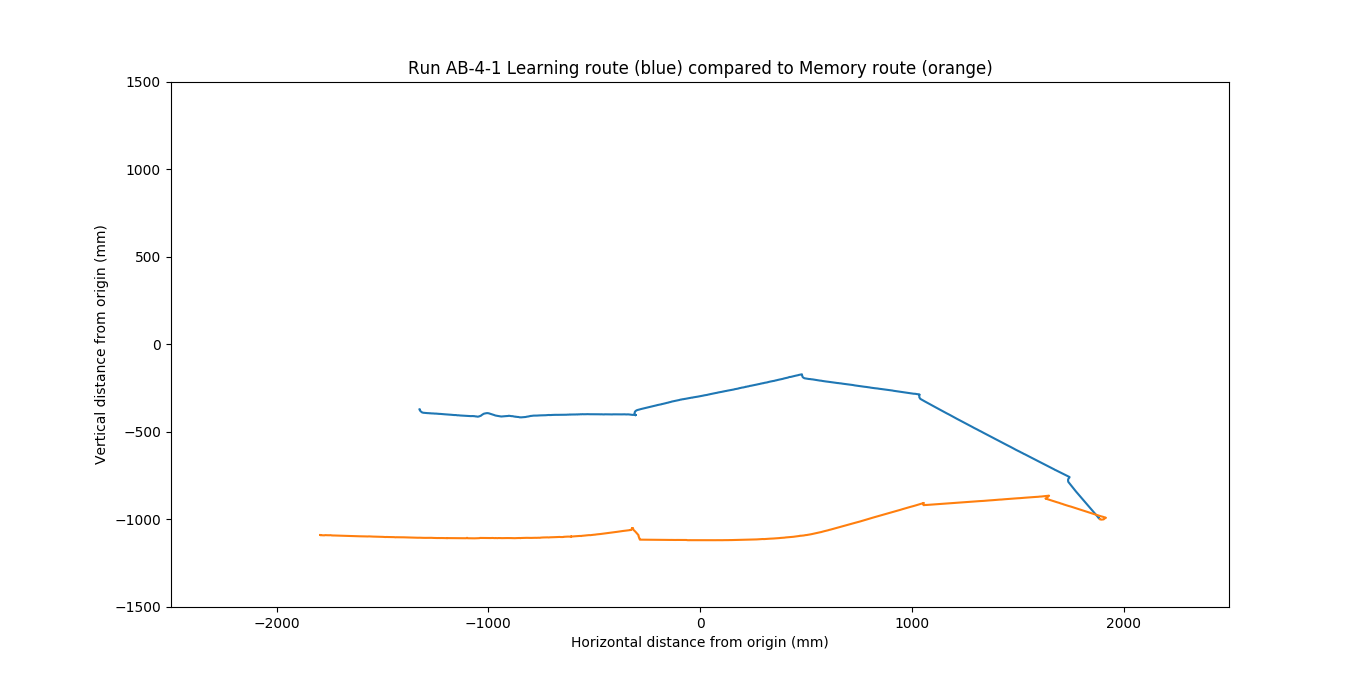
\includegraphics[width=\textwidth]{AB-4-1}
  \caption{
    \label{fig:ab-4-1-fail} Trajectory plot of run AB-4-1; this run was considered a failure of the
    Visual Navigation system.
  }
\end{figure}

We also see some more successful navigation in runs such as AB-3-1 (shown in Figure \ref{fig:ab-3-1-succ}). It should first be
noted that, once reaching a spot near the end of the learned route, the visual navigation would struggle as it had no
more information to work from; this is simply due to the timed nature of experiments. We are interested quite simply in how
closely the recalled route follows the learned route. 

\begin{figure}
 \centering
  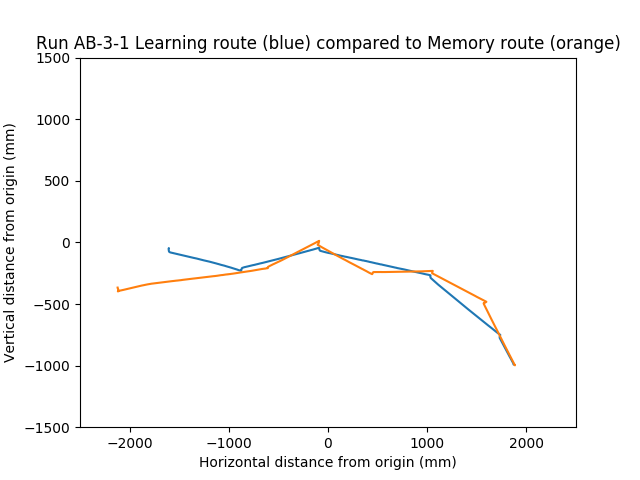
\includegraphics[width=\textwidth]{AB-3-1}
  \caption{
    \label{fig:ab-3-1-succ} Trajectory plot of run AB-3-1; this run was considered a success of the Visual Navigation
    system.
  }
\end{figure}

Figure \ref{fig:ab-3-1-succ} demonstrates the ideal behaviour wherein the robot zig-zags over the correct route, consistently
correcting to keep itself on course. It is in this behaviour we see the model's capacity to remember the visual corridor
correctly. We do occassionally observe another behaviour; the robot will lose its way and recover. This behaviour occurred in
cases where the robot was lucky enough to get a view which would allow it to correct. There were cases which looked as if
they were correcting, however, they failed to recover the route. Examples of both can be seen in Figures \ref{fig:ab-2-2-succ}
and \ref{fig:mab-1-2-succ} respectively. In particular Figure \ref{fig:ab-2-2-succ} highlights a problem with the timed
nature of the experiments. Though it appears the robot will recover, there is no way of knowing for sure.
The timer is used as there is no real way to distinguish memories of home and food source from memories of the route using
the current model. We should also note that using timers on the robot caused a great deal of inconsistency in general; during
recapitulation of AB runs, the robot was meant to move for a time interval of 2 \textit{seconds}, during MAB experiments, this
interval was reduced to 1 \textit{second}. It can clearly be seen from the trajectory plots that the robot did not move in
consistent intervals during recapitulation. A potential solution to this problem is to use the \textit{move()} command to
move a set distance, however, this has potential to cause problems with the CA system.

\begin{figure}
 \centering
  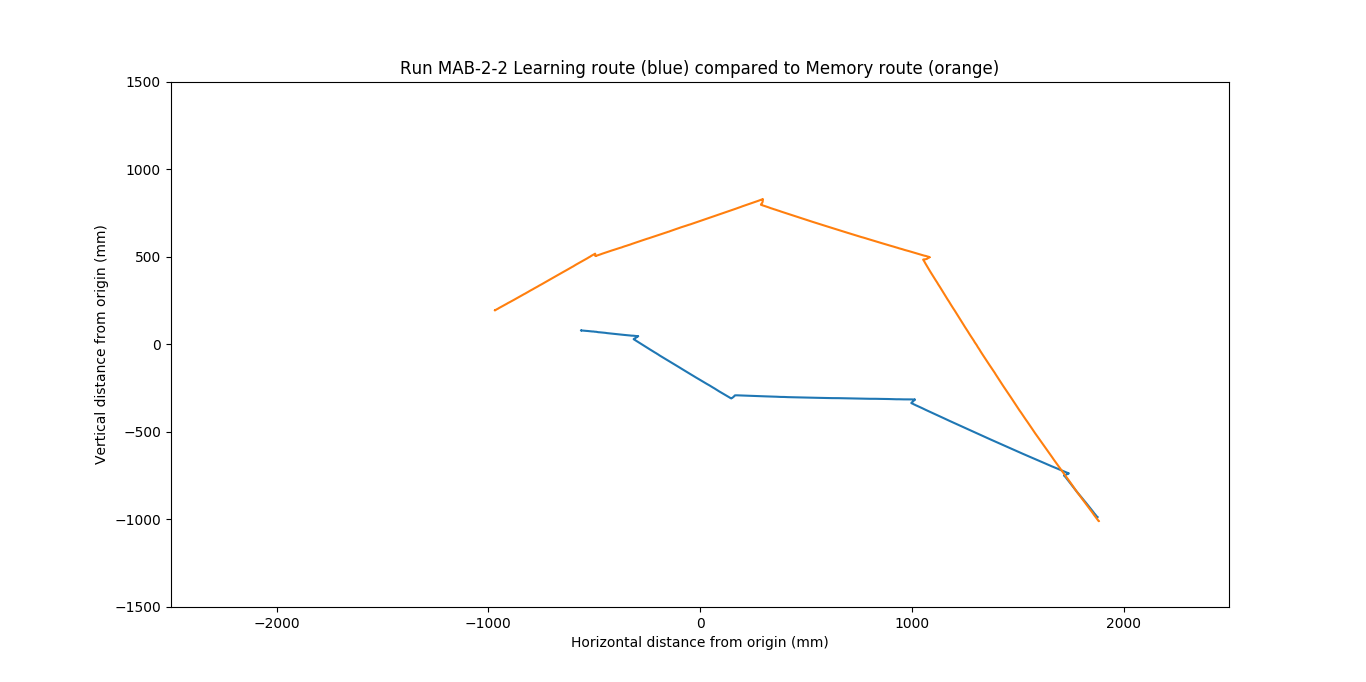
\includegraphics[width=\textwidth]{MAB-2-2}
  \caption{
    \label{fig:mab-2-2-succ} Trajectory plot of run AB-1-2; a near-successful recovery.
  }
\end{figure}


\begin{figure}
 \centering
  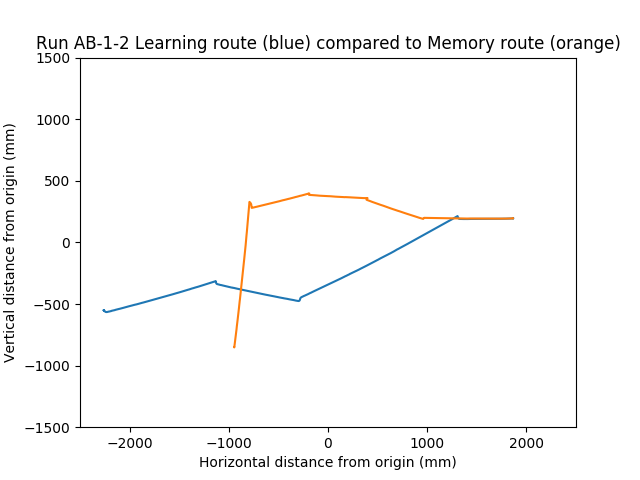
\includegraphics[width=\textwidth]{AB-1-2}
  \caption{
    \label{fig:ab-1-2-fail} Trajectory plot of run AB-1-2; a failed recovery.
  }
\end{figure}

It was mentioned in Section \ref{sec:test} that the behaviour of the robot during learning was modified slightly. This
was due to the type of behaviour we see in Figure \ref{fig:ab-3-2}. This run was considered successful, however it can be seen
that the robot did not follow the route precisely, rather following an inside line. A potential reason was seen as the
delay between obstacle detection and reaction during learning. Along with the increased image count, the runs from
the modified learning system (tagged MAB) performed better in general, however there were certainly still errors.
\newline

\begin{figure}
 \centering
  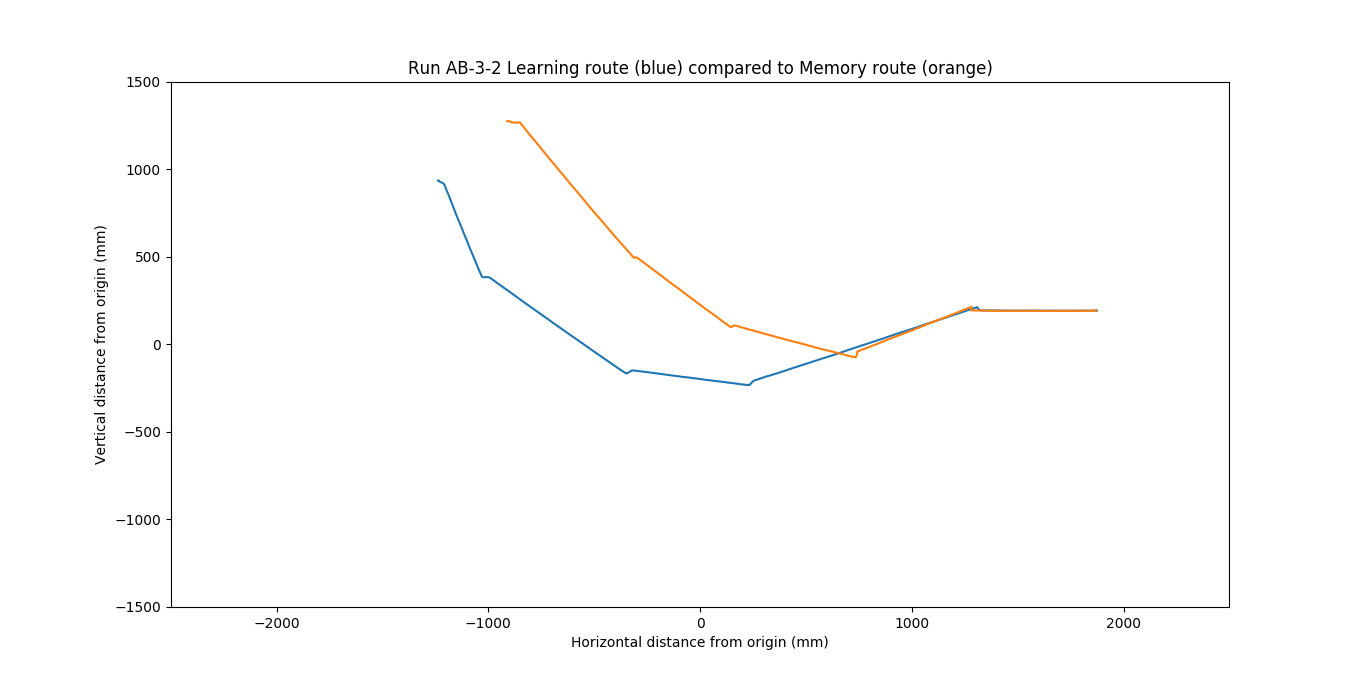
\includegraphics[width=\textwidth]{AB-3-2}
  \caption{
    \label{fig:ab-3-2} Trajectory plot of run AB-3-2.
  }
\end{figure}

In all, the visual navigation system performed quite well. Drastic errors were rare, though certainly present.The full series
of trajectories in Appendix \ref{app:plots} show that the network was capable of reproducing routes on a robot through a
cluttered (yet low detail due to the distorted field of vision) environment using a visual scanning route following behaviour.
\newline

What follows was not a formal experiment, but rather an exercise in curiosity. We gave AntBot the ability to learn homeward
routes by rotating each image by $180^{\circ}$ and storing both the original and rotated versions. The robot was then set
to run a learning route through an empty arena and tasked with retracing its route home, then back out, and so on. Two runs
of this nature were conducted, however, only one was recorded. During the first run, the arena contained a box and the
robot did not cope well with this landscape; outbound routes performed as well as could be expected, though inbound routes
failed badly, requireing numerous corrections. The second run (taking place in the empty arena) faired far better, though
corrections were still required. The trajectories can be seen in Figure \ref{fig:home}. Two corrections were required
through the course of these experiments during runs \textit{Memory 1} and \textit{Memory 5}. Both corrections occurred
at an offset of greater than 2000mm (in the negative direaction) from the origin and, once corrected, the robot successfully
navigated home. There was one out of three homeward routes that  

\begin{figure}
 \centering
  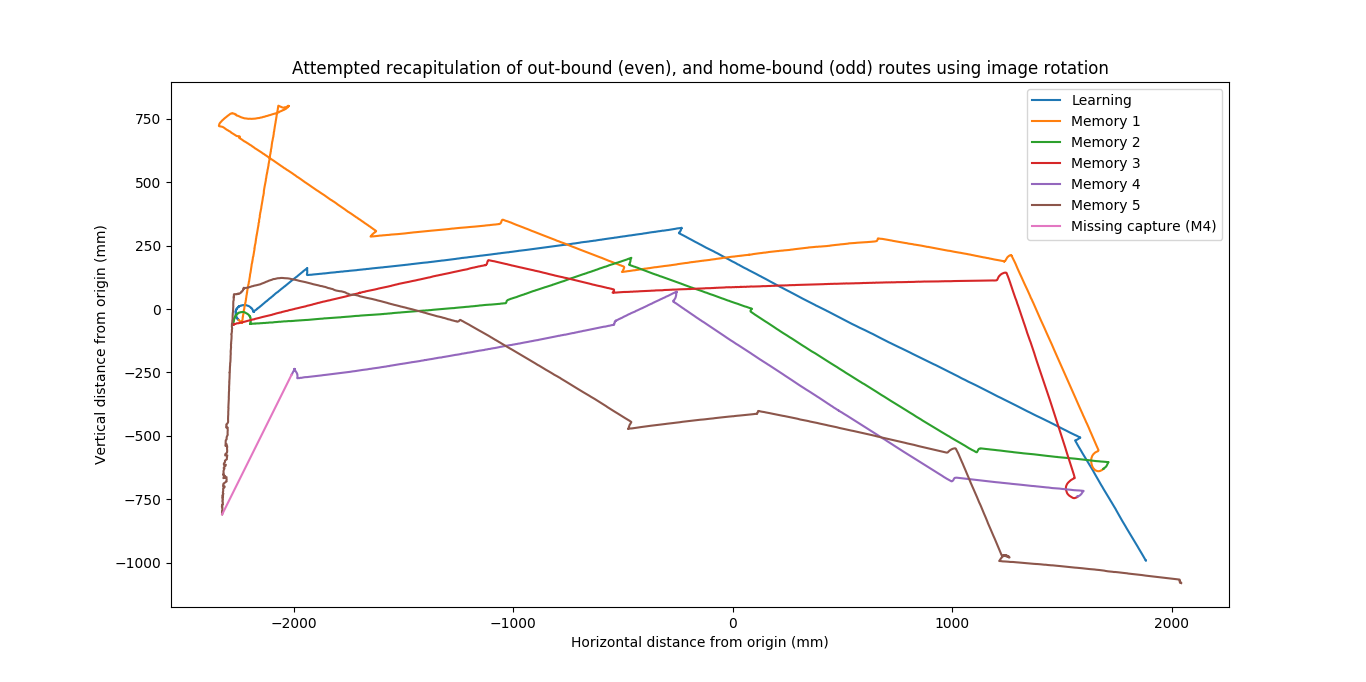
\includegraphics[width=\textwidth]{Homeward}
  \caption{
    \label{fig:home} Trajectory plot of the homeward experiment. The Vicon capture was accidentally stopped
    early during outward trip \textit{Memory 4} and the last section of the trip was missed. The linkage has
    been filled in to show where the rough route the robot took but it must be understood that this is not
    part of the recording, the line was simply drawn to fill in the gap. 
  }
\end{figure}

\newpage

\section{ Discussion } \label{sec:discussion}
\subsection{Conclusion}
In this project, we have investigated the plausibility of a visual collision avoidance system based on optical flow combining
this with a visual navigation model using the Mushroom Body. We investigated two different optical flow based collision avoidance
systems and found results indicating the impracticality of a time-to-collision/depth centric system on the current robot. We
also presented here results which show that even a basic flow filter based system can function well, though is certainly
not without its flaws. We then investigated the Mushroom Body circuit for visual navigation, undertaking the debugging
process to find out why the network seemingly did not function as it should. In the end, the problem with the visual
navigation was found to be the route following strategy which was failing as a result of the control system implementation. We
implemented a visual scanning algorithm for the robot and saw a drastic improvement in the functionality of the navigation
system. Results presented for the Mushroom Body demonstrate a clear capacity for route memory in the context of a ``visual
corridor'' allowing the robot to navigate in the manner observed in ants. While we have seen improvement in the performance
of the MB model, we do still present many cases where the robot became confused, or chose its direction incorrectly. We will
present ideas for future improvement in the following section.

\subsection{Future work}
\subsubsection{Improvements on work presented}
Here we wish to draw attention to the flaws in the experiments or research presented here and propose solutions.
\newline

Firstly, we wish to discuss time-to-contact and image depth. While the methods presented did not work, there are
some modifications that could be made to gain a functioning system. We know that the system struggles to cope
with a dense flow field, yet the points returned by the \textit{goodFeaturesToTrack()} result in inconsistency. We
could however take a subset of a dense flow field to reduce the computational demand, yet maintain the stability of
considering set points in the frame. The flow field was not the only problem in computing time-to-contact. We also
need the translational velocity of the camera. \textit{Scimeca} found that a dense flow field was far better at
computing accurate speed information than a sparse field, however, only one field may be in use on the robot at
a single time. Introducing a subset system would allow us to use the dense flow information to compute the speed
which gives us a more accurate estimation of time-to-contact. Alternatively, wheel encoders could be used to compute the
speed information \textit{[NOTE: STEPCOUNTING]}.
\newline

We note also that AntBot's field of vision is greatly distorted and while the tussocks may seem to completely
fill the camera view, in reality, they are providing minimal detail. This could quite easily be remedied by
constructing taller tussocks which provide more detail. We think that this could have a great effect on the
performance of the VN and CA systems here presented.
\newline

 
\subsubsection{Hardware engineering}

\newpage

\bibliographystyle{plain}
\bibliography{working}
\newpage

\appendix
\section{Visual Navigation trajectory plots} \label{app:plots}
\textit{Plots to follow...}

\end{document}




